\PassOptionsToPackage{unicode=true}{hyperref} % options for packages loaded elsewhere
\PassOptionsToPackage{hyphens}{url}
%
\documentclass[]{article}
\usepackage{lmodern}
\usepackage{amssymb,amsmath}
\usepackage{ifxetex,ifluatex}
\usepackage{fixltx2e} % provides \textsubscript
\ifnum 0\ifxetex 1\fi\ifluatex 1\fi=0 % if pdftex
  \usepackage[T1]{fontenc}
  \usepackage[utf8]{inputenc}
  \usepackage{textcomp} % provides euro and other symbols
\else % if luatex or xelatex
  \usepackage{unicode-math}
  \defaultfontfeatures{Ligatures=TeX,Scale=MatchLowercase}
\fi
% use upquote if available, for straight quotes in verbatim environments
\IfFileExists{upquote.sty}{\usepackage{upquote}}{}
% use microtype if available
\IfFileExists{microtype.sty}{%
\usepackage[]{microtype}
\UseMicrotypeSet[protrusion]{basicmath} % disable protrusion for tt fonts
}{}
\IfFileExists{parskip.sty}{%
\usepackage{parskip}
}{% else
\setlength{\parindent}{0pt}
\setlength{\parskip}{6pt plus 2pt minus 1pt}
}
\usepackage{hyperref}
\hypersetup{
            pdftitle={Is the London Cycle Hire Scheme becoming more inclusive? An evaluation of the shifting spatial distribution of uptake based on 70 million trips},
            pdfborder={0 0 0},
            breaklinks=true}
\urlstyle{same}  % don't use monospace font for urls
\usepackage[margin=1in]{geometry}
\usepackage{longtable,booktabs}
% Fix footnotes in tables (requires footnote package)
\IfFileExists{footnote.sty}{\usepackage{footnote}\makesavenoteenv{longtable}}{}
\usepackage{graphicx,grffile}
\makeatletter
\def\maxwidth{\ifdim\Gin@nat@width>\linewidth\linewidth\else\Gin@nat@width\fi}
\def\maxheight{\ifdim\Gin@nat@height>\textheight\textheight\else\Gin@nat@height\fi}
\makeatother
% Scale images if necessary, so that they will not overflow the page
% margins by default, and it is still possible to overwrite the defaults
% using explicit options in \includegraphics[width, height, ...]{}
\setkeys{Gin}{width=\maxwidth,height=\maxheight,keepaspectratio}
\setlength{\emergencystretch}{3em}  % prevent overfull lines
\providecommand{\tightlist}{%
  \setlength{\itemsep}{0pt}\setlength{\parskip}{0pt}}
\setcounter{secnumdepth}{5}
% Redefines (sub)paragraphs to behave more like sections
\ifx\paragraph\undefined\else
\let\oldparagraph\paragraph
\renewcommand{\paragraph}[1]{\oldparagraph{#1}\mbox{}}
\fi
\ifx\subparagraph\undefined\else
\let\oldsubparagraph\subparagraph
\renewcommand{\subparagraph}[1]{\oldsubparagraph{#1}\mbox{}}
\fi

% set default figure placement to htbp
\makeatletter
\def\fps@figure{htbp}
\makeatother


\title{Is the London Cycle Hire Scheme becoming more inclusive? An evaluation of the shifting spatial distribution of uptake based on 70 million trips}
\author{}
\date{\vspace{-2.5em}}

\begin{document}
\maketitle

{
\setcounter{tocdepth}{2}
\tableofcontents
}
\hypertarget{abstract}{%
\section*{Abstract}\label{abstract}}
\addcontentsline{toc}{section}{Abstract}

Pro-cycling interventions, and cycle hire schemes in particular, are often assumed to primarily benefit the privileged.
This framing has played-out in academic research, with many papers exploring the relationship between cycling and existing inequalities.
A growing body of evidence suggests that cycle hire schemes tend serve wealthy areas and young, high income groups, mirroring inequalities in other types of cycling uptake, yet there has been little research into the `direction of travel' and whether such inequalities are growing or `levelling up' over time.
This paper explores the uptake of the London Cycle Hire Scheme (LCHS), a large, early and prominent scheme that had the explicit aim of `normalising' cycling.
The method involved analysis of 73.4 million cycle high records spanning 8 years from January 2012 to December 2020, using the geographic location of docking stations alongside official statistics to assess social and spatial inequalities in uptake.
We found that, contrary to the trend for increasing segregation and geographic inequalities, the usage of the LCHS have become increasingly geographically distributed across London over time, with AM peak usage in comparatively low-income areas seeing high levels of growth.
Our study shows that cycle hire schemes can be designed and expanded in ways that benefit a wide range of people, including those from low income areas, and that new cycle hire docking stations in poorer areas can succeed.

\hypertarget{introduction}{%
\section{Introduction}\label{introduction}}

Since the turn of the 21\textsuperscript{st} Century, cycling has risen to prominence in transport plans worldwide.
Once perceived as an old fashioned mode, recent evidence on its ability to support pressing political priorities --- including air quality, congestion, liveable streets, and health/well-being --- has led to policies explicitly enabling cycling uptake in many cities including Beijing, New York, Santiago and London.

Bike share schemes (BSS) such as the LCHS aim to address two of the major barriers to cycling: lack of access to a working bike and the perception that cycling is only for certain (often young, male, high income) groups by providing 24/7 access to bikes at relatively low costs (compared with motorised modes, and driving a private automobile in particular) (Shaheen, Guzman, and Zhang 2012), enabling a wide range of people to access the benefits of cycling (Goodman, Green, and Woodcock 2014).
BSSs are inevitably localised policies, enabling bikes to be rented at multiple docking stations located across (usually central) parts of cities, especially near major trip attractors, and the data they produce provides a rich source of information on how cycling levels are changing and shifting (O'Brien et al. 2014).

Cycle hire is a rapidly evolving phenomenon.
The first schemes allowed the use of bicycles for free (`First generation'), or through a coin deposit (`Second generation'), which often resulted in problems of financing and theft.
The `Third generation' schemes, to which the LCHS belongs, allow users to access and return bikes to dedicated docking stations, typically with only a bank card or other type of payment device, which makes the service more viable.
`Fourth generation' smart bikes with integrated locking technology can communicate with user smart phone apps, removing the need to communicate with a station or terminal, enabling journeys to start or end away from traditional docking stations.
This free-floating operational `dockless' bikeshare model, can also run as a hybrid model composed of docking stations and free-floating parking zones shown on a map (Li et al. 2019).

Globally, there has been an emergence of schemes funded primarily by private capital and with lower installation times, accounting for the majority of growth in bike share fleets worldwide since 2016 (Fishman and Schepers 2018).
Continued growth and the private capital led operations makes assessment of bikeshare important, to monitor their performance compared with other types of sustainable transport intervention, understand how bikeshare is used, where and by whom and to ensure that future cycle hire policies support, rather than hinder, local policy objectives.
While Fourth generation schemes have seen explosive growth in some areas, they have also suffered setback, including the high-profile collapse of dockless bike companies leading to questions about the sustainability of Fourth generation schemes (Nikitas 2019) and the docked bikes of the LCHS still dominate the local market.

In this context the aim of this paper is to better understand the extent to which cycle hire schemes have been adopted by users from areas of differing socio-economic outcomes.
Using data from the London Cycle Hire Scheme (LCHS), first launched in 2010 and continuously expanded since, we explore usage patterns in high and low income areas.
After a review of literature on the growth of cycle hire from a social equity perspective (Section 2), the paper describes the LCHS in detail (Section 3), outlines methods for comparing usage levels over time across geographic areas (Section 4), and presents the findings (Section 5).
The final sections discuss the findings in relation to pressing policy and research questions and conclude with recommendations for transport policymakers and researchers.

\hypertarget{background}{%
\section{Background}\label{background}}

Bicycle sharing systems (BSS) have been created in many cities to support multiple policy objectives, especially improved health, air quality and liveability (Fishman 2016).
Modern docked cycle hire schemes have been in operation since 1995, with the launch of a scheme in Copenhagen (DiDonato, Herbert, and Vachhani 2002).
They have taken off since the early 2000s, with the greatest absolute period of growth occurring between around 2010 and 2015, after which the rate of new installations has dropped off (Figure \ref{fig:global-growth}).

\begin{figure}[h]

{\centering 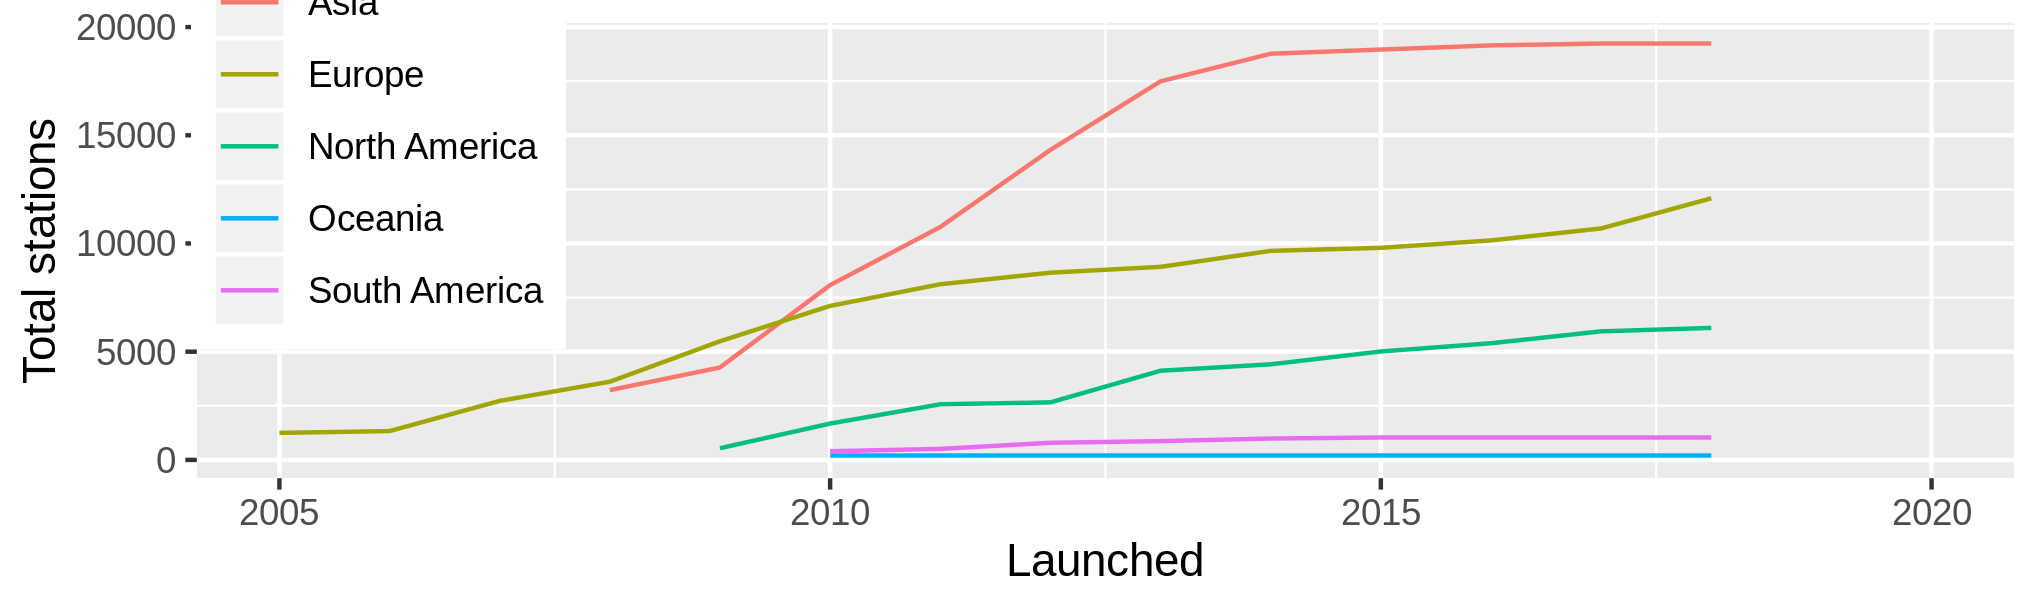
\includegraphics[width=0.8\linewidth]{figures/bikehshare-global-stations-growth} 

}

\caption{Growth in docked cycle hire schemes worldwide in terms of docking stations by continent.}\label{fig:global-growth}
\end{figure}

European cities pioneered shared cycle mobility, with schemes in cities such as Amsterdam (The Netherlands) and Rennes (France) demonstrating the concept's feasibility (DiDonato, Herbert, and Vachhani 2002), and the number of European schemes has continued to grow.
Asia saw very rapid uptake of sharing schemes from 2010. Seven of the top ten largest schemes by number of docking stations and number of bicycle have been launched in Chinese cities between 2008 and 2011 (see Figure \ref{fig:global-stations-cycles}).
North and South America have seen substantial interest in docked cycle hire schemes, although on a smaller scale than those in Europe and Asia, and a handful of cycle hire schemes have been launched in Australia.
Within this global overview, the London BSS is an important player, ranking eighth in the top schemes by number of docking stations and launching relatively early in 2010.

\begin{figure}[h]

{\centering 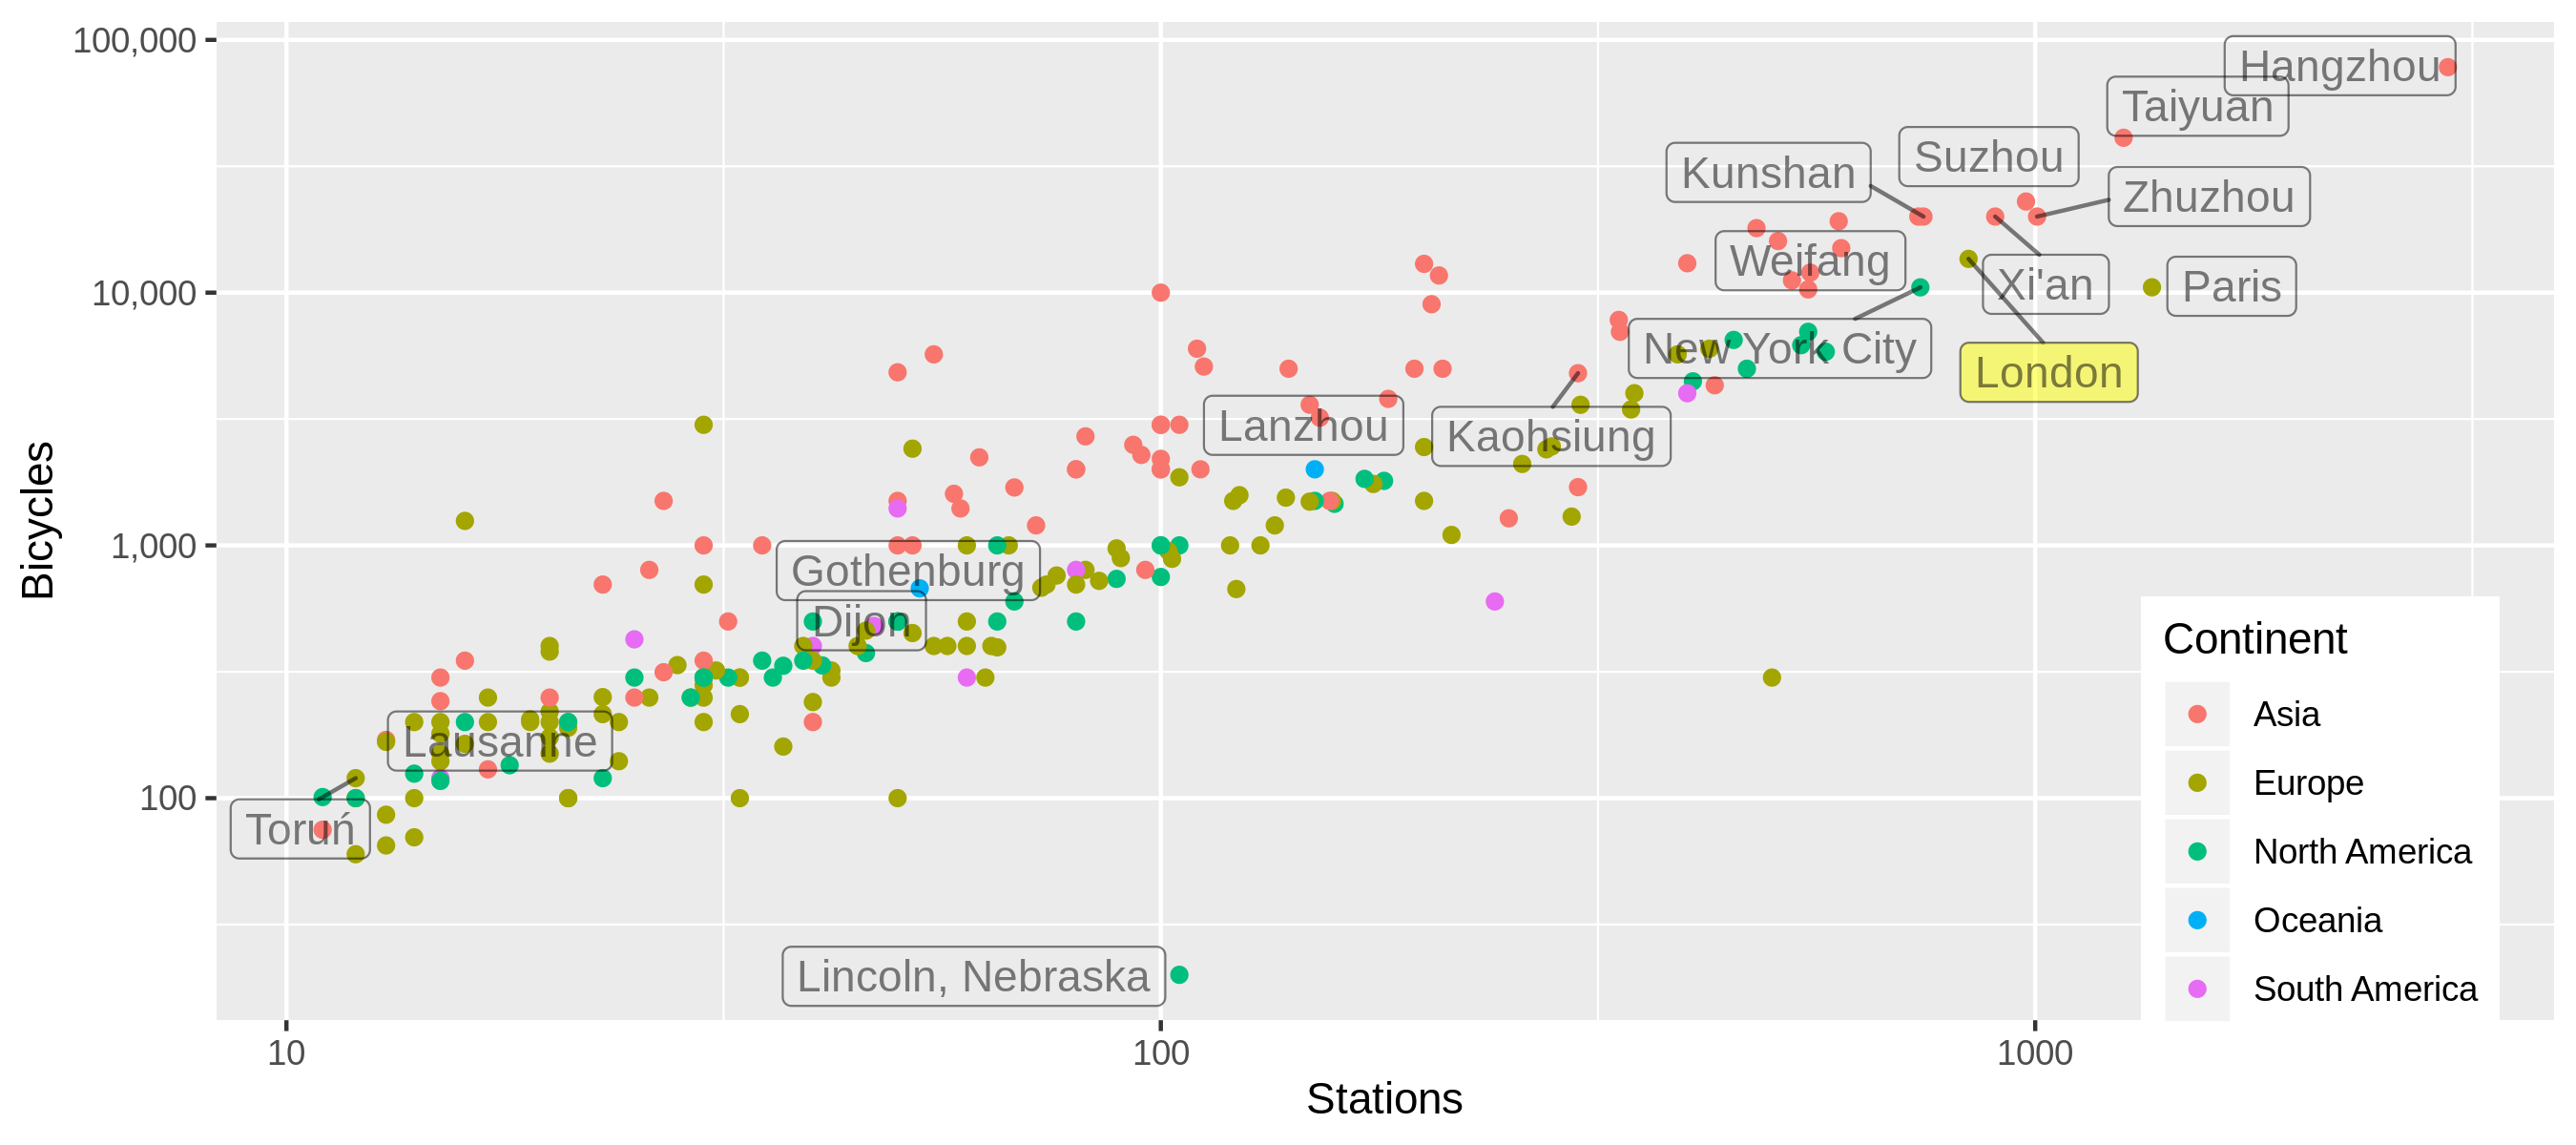
\includegraphics[width=0.8\linewidth]{figures/bikehshare-global-stations-bicycles} 

}

\caption{Cycle hire schemes worldwide by continent, comparing number of docking stations with number of cycles.}\label{fig:global-stations-cycles}
\end{figure}

\hypertarget{determinants-of-cycle-hire-scheme-usage}{%
\subsection{Determinants of cycle hire scheme usage}\label{determinants-of-cycle-hire-scheme-usage}}

\hypertarget{who-uses-cycle-hire-schemes}{%
\subsubsection{Who uses cycle hire schemes?}\label{who-uses-cycle-hire-schemes}}

Much research has been devoted to the question of who uses BSS.
In general, reflecting cycle usage overall, BSS users appear to be younger adults, have higher incomes than average, male and are more likely to own a bicycle (Ogilvie and Goodman 2012; Fishman, Washington, and Haworth 2013; Zhao et al. 2019; Soltani et al. 2019; Heinen, Kamruzzaman, and Turrell 2018).
These socio-economic characteristics may seem similar to those that are generally linked to cycling (see e.g. Heinen, Wee, and Maat 2010).

However, some research reveals certain differences between cyclists using BSS and `normal' cyclists that imply BSS can open up cycling to a wider range of users.
Buck et al. (2013, 112) found in the Washington, D.C., region that, compared with regular cyclists, bike-share users ``are more likely female, younger, have lower household incomes, own fewer cars and fewer bicycles, and are more likely to cycle for utilitarian trip purposes''.

\hypertarget{where-are-hired-cycles-used}{%
\subsubsection{Where are hired cycles used?}\label{where-are-hired-cycles-used}}

Research has focussed on where users ride, partly perhaps driven by an underlying question of where stations are best placed. BSS stations that are located in either a city centre and on a university campus are often well used (Mattson and Godavarthy 2017; Zhang et al. 2016).
Other facilities have been shown to increase use of bicycle sharing stations, including proximity to housing, train and metro stations, bus stops, shops, parks, hospitals, and employment sites (Fishman, Washington, and Haworth 2014; Bachand-Marleau, Lee, and El-Geneidy 2012; Buck et al. 2013; Daddio and Mcdonald 2012; Wang and Lindsey 2019; Rixey 2013; Nair et al. 2013; Hampshire and Marla 2012; Fuller et al. 2011; Zhao et al. 2019; Mooney et al. 2019).

Cycling organisations have advocated that BSS stations should be located not only on their potential use, but also on their potential to provide new mobility options to disadvantaged transport populations (League of American Bicyclists and Club 2015; Sustrans 2019).
In Boston, Chicago, Denver, Seattle, and New York City (US), Aultman-Hall and Ursaki (2015) found significant differences in access based on race and income variables.
In Porto Alegre, Recife, Rio, Salvador and Sao Paulo (Brazil), Duran et al. (2018) found that the coverage of bicycle-sharing systems favoured wealthier and centrally located neighborhoods with higher proportion of white population.

\hypertarget{bicycle-sharing-schemes-transport-equity-and-social-inclusion}{%
\subsection{Bicycle sharing schemes, transport equity and social inclusion}\label{bicycle-sharing-schemes-transport-equity-and-social-inclusion}}

BSS have the potential to enable a wider range of people to benefit from access to cycling for daily transport as it offers an affordable form of transport.
The LCHS costs £2 for making a potentially unlimited number of rides of less than 30 minutes over a 24 hour period of use, for example which is less than half the price of a typical single use metro (tube) ticket.\footnote{See \url{https://tfl.gov.uk/modes/cycling/santander-cycles/what-you-pay} and \url{https://tfl.gov.uk/fares/find-fares/tube-and-rail-fares} for cycle hire and tube prices respectively.}
However, the lowest rates, such as the £90 for an annual ticket bought online, may exclude those on low incomes.
Another benefit of accessing a bike through a BSS is that maintenance and storage are paid for by the operator. Bike theft represents another potential problem that can be mitigated by cycle hire schemes.
All these may be of greater importance in low income areas, where the barriers to buying, storing, repairing, and bike theft will likely be greater.
A study on barriers to bikeshare on traditionally under-served neighbourhoods in the US (Portland State University et al. 2017, 1) found that some of the most common barriers to bicycling cited by lower-income people of color were issues that bike share could address, such as: not having a bike or related gear (47\%); not having a safe place to leave a bike where they need to go (36\%); the expense of buying a bike or related gear (41\%); and not having a safe place to store a bike at home (32\%).
Inequalities related to BSS are directly linked to use and access, and the consequent benefits of accessibility -- health.

As discussed in the preceding paragraphs, BSS tends to be associated with higher socio-economic groups and higher incomes.
However, the use of schemes is also dependent on other aspects of social disadvantage.
Transport for London (TfL 2016), for example, found that casual users generally have lower incomes than annual members, implying that users with higher incomes would make more use of economically beneficial long-term subscriptions.
Similarly, Ogilvie and Goodman (2012) reported that registered users of the London scheme were more likely living in socio-economically advantaged areas, indicating that they may also have higher disposable income.
Other studies indicated that users are most likely to be middle-class (Clark and Curl 2016).
Interestingly, the use of the scheme among registered users of the LCHS has been found to be more common for individuals living in more deprived areas: they made more trips than individuals in wealthier areas according to Ogilvie and Goodman (2012), suggesting different dynamics than those identified in studies of American BSS.
A recent example in Glasgow also demonstrates that BSS can gain high uptake among disadvantaged groups, provided sufficient support.
The `\href{https://www.nextbike.co.uk/en/news/nextbike-provides-bikes-for-all-as-scheme-celebrates-community/}{Bikes for All}' BSS scheme was supported by a parallel package of engagement activities and measures to overcome barriers (particularly financial barriers) to shared mobility faced by diverse groups including along ethnic, housing tenure and employment lines.
The results from follow-up research into the scheme's impact shows that providing additional support, in addition to simply putting shared bikes in low income areas, can ensure high uptake among a wide range of disadvantaged groups (Yates and Whyte 2019).\footnote{The scheme attracted a diversity of demographics, 49\% identified as Black or Minority Ethnicity (BME), 26\% were seeking asylum, 28\% were unemployed, 42\% were women and 9\% were homeless.}

Accessibility to and awareness of BSS is also not equally spread across the population.
Areas with no docking stations have been found to have lower levels of awareness of shared mobility as a transport option (Bernatchez et al. 2015).
BSSs tend to be more easily accessible to higher socio-economic groups (e.g. Ricci 2015) and one reason offered for this is that stations may not be placed in less economically advantaged areas.
Ogilvie and Goodman (2012) reported that registered users of the London scheme were more likely to live in socio-economically advantaged areas and areas with high cycling levels.

Overall, there is little evidence of the transport equity outcomes from cycle hire schemes.
One recent paper on the role of cycle hire schemes in transport equity, stated that ``most BSS typically benefit the privileged'' (Chardon 2019, 401).
In the same direction, Noland (2018, 151) found in Philadelphia that ``bikeshare docking stations in lower income areas are not generating as many trips as in other areas''.
Hosford and Winters (2018) noted the importance of confounding geographic factors: economically advantaged areas have better access in some cities, whereas in other cities disadvantaged areas are better served.
Nevertheless, these studies are cross-sectional and provide little insight into the direction of travel in terms of increasing or decreasing levels of inequality in cycle hire use over time.

\hypertarget{the-london-cycle-hire-scheme}{%
\section{The London Cycle Hire Scheme}\label{the-london-cycle-hire-scheme}}

With an urban population approaching 9 million, London is the largest city in Western Europe and, housing many the world's `super rich', has substantial overseas links (Shrubsole 2019).
In addition to economic and cultural influence associated with the super-rich (a driver of high living costs and economic inequalities), London's status as an international financial hub and cosmopolitan study and tourist destination boosts the city's `soft power' (Bell 2016).\footnote{Although Bell (2016) is focussed on the British influence, many of the paper's main points are particularly relevant to London.
  In terms of tourism, London attracts \textasciitilde{}30 million visitors each year according \href{http://www.uncsbrp.org/tourism.htm}{London's Economic Plan}.}
On seeing and trying accessible cycling, some of London's diverse and generally wealthy visitors may go on to try cycling elsewhere.

Unlike other major high-income cities in the UK (and the world), the majority of trips in the UK's capital are made by `sustainable' modes, with public transport, walking and cycling accounting for 35\%, 24\% and 2\% of trips in 2016 respectively, although cars still account for around 35\% of trips, according to London's \href{https://www.google.com/url?sa=t\&rct=j\&q=\&esrc=s\&source=web\&cd=5\&ved=2ahUKEwjj6b6pldXlAhV5ShUIHRQZBYQQFjAEegQIAhAC\&url=https\%3A\%2F\%2Ftfl.gov.uk\%2Fcdn\%2Fstatic\%2Fcms\%2Fdocuments\%2Ftravel-in-london-report-10-data.xlsx\&usg=AOvVaw3wFwZPyKmV86i71fCoa0Bo}{10}s Travel report).
Cycling is the fastest growing mode of transport in London, with trip numbers more than doubling since 2000.\footnote{See \url{https://www.london.gov.uk/sites/default/files/londons_cycling_infrastructure.pdf}}

LCHS has a direct impact on many London residents who have used the scheme since its 2010 launch (making London an early adopter).
It is large, boasting the second largest number of bikes of any system worldwide in 2014 (Fishman 2016).\footnote{There were nearly 10,000 bikes in the scheme at the time and there are around 11,500 now, although fewer are in circulation, docked or being used on the streets.
  According to data from \href{https://bikesharemap.com/london/\#/12.384657071672539/-0.1195/51.5021/}{bikesharemap.com} there are around 8,000 cycles typically in circulation.
  See \url{https://madeby.tfl.gov.uk/2019/08/09/cycle-hire-trivia-and-facts/} for more cycle hire facts and figures.}
The stated aim was to provide ``a major new form of public transport in London, delivering an additional 40,000 cycle trips per day'' (Transport for London 2010) (currently the scheme averages 30,000 hires per day over the year, around double the initial level of usage, with peaks over 45,000 trips on busy summer days).
Although the scheme currently delivers only around 0.1\% of trips in Greater London overall, it serves a much higher percentage of trips in the congested central areas during the vital rush hours.
By providing a new form of transport targeting commuters, another important aim was to relieve peak capacity constraints on the tube and bus network\footnote{`We want thousands of commuters to switch to bikes for the last stage of their journeys to work, significantly relieving pressure on the Tube and bus networks in central London.' \url{https://www.london.gov.uk/sites/default/files/cycling_vision_gla_template_final.pdf}}. It should be noted that in recent years new bikeshare operators have established themselves in London, many of which offering more flexible dockless usage.
Analysis by Li et al. (2019) suggests that new opperators have reduced usage of the LCHS, especially for short trips and during times of peak demand.
These schemes offer exciting opportunities for analysis --- many contain in-built GPS recording users' full journey trajectories --- the Santander scheme remains by far the largest and most widely used scheme in London, as shown in Figure \ref{fig:cycle-hire-players}.
In the absence of data on dockless hire cycle usage, and considering that that the aim of the present paper is to assess \emph{relative} changes between docking stations (not overall demand) we keep the focus on open LCHS data.

\begin{figure}

{\centering 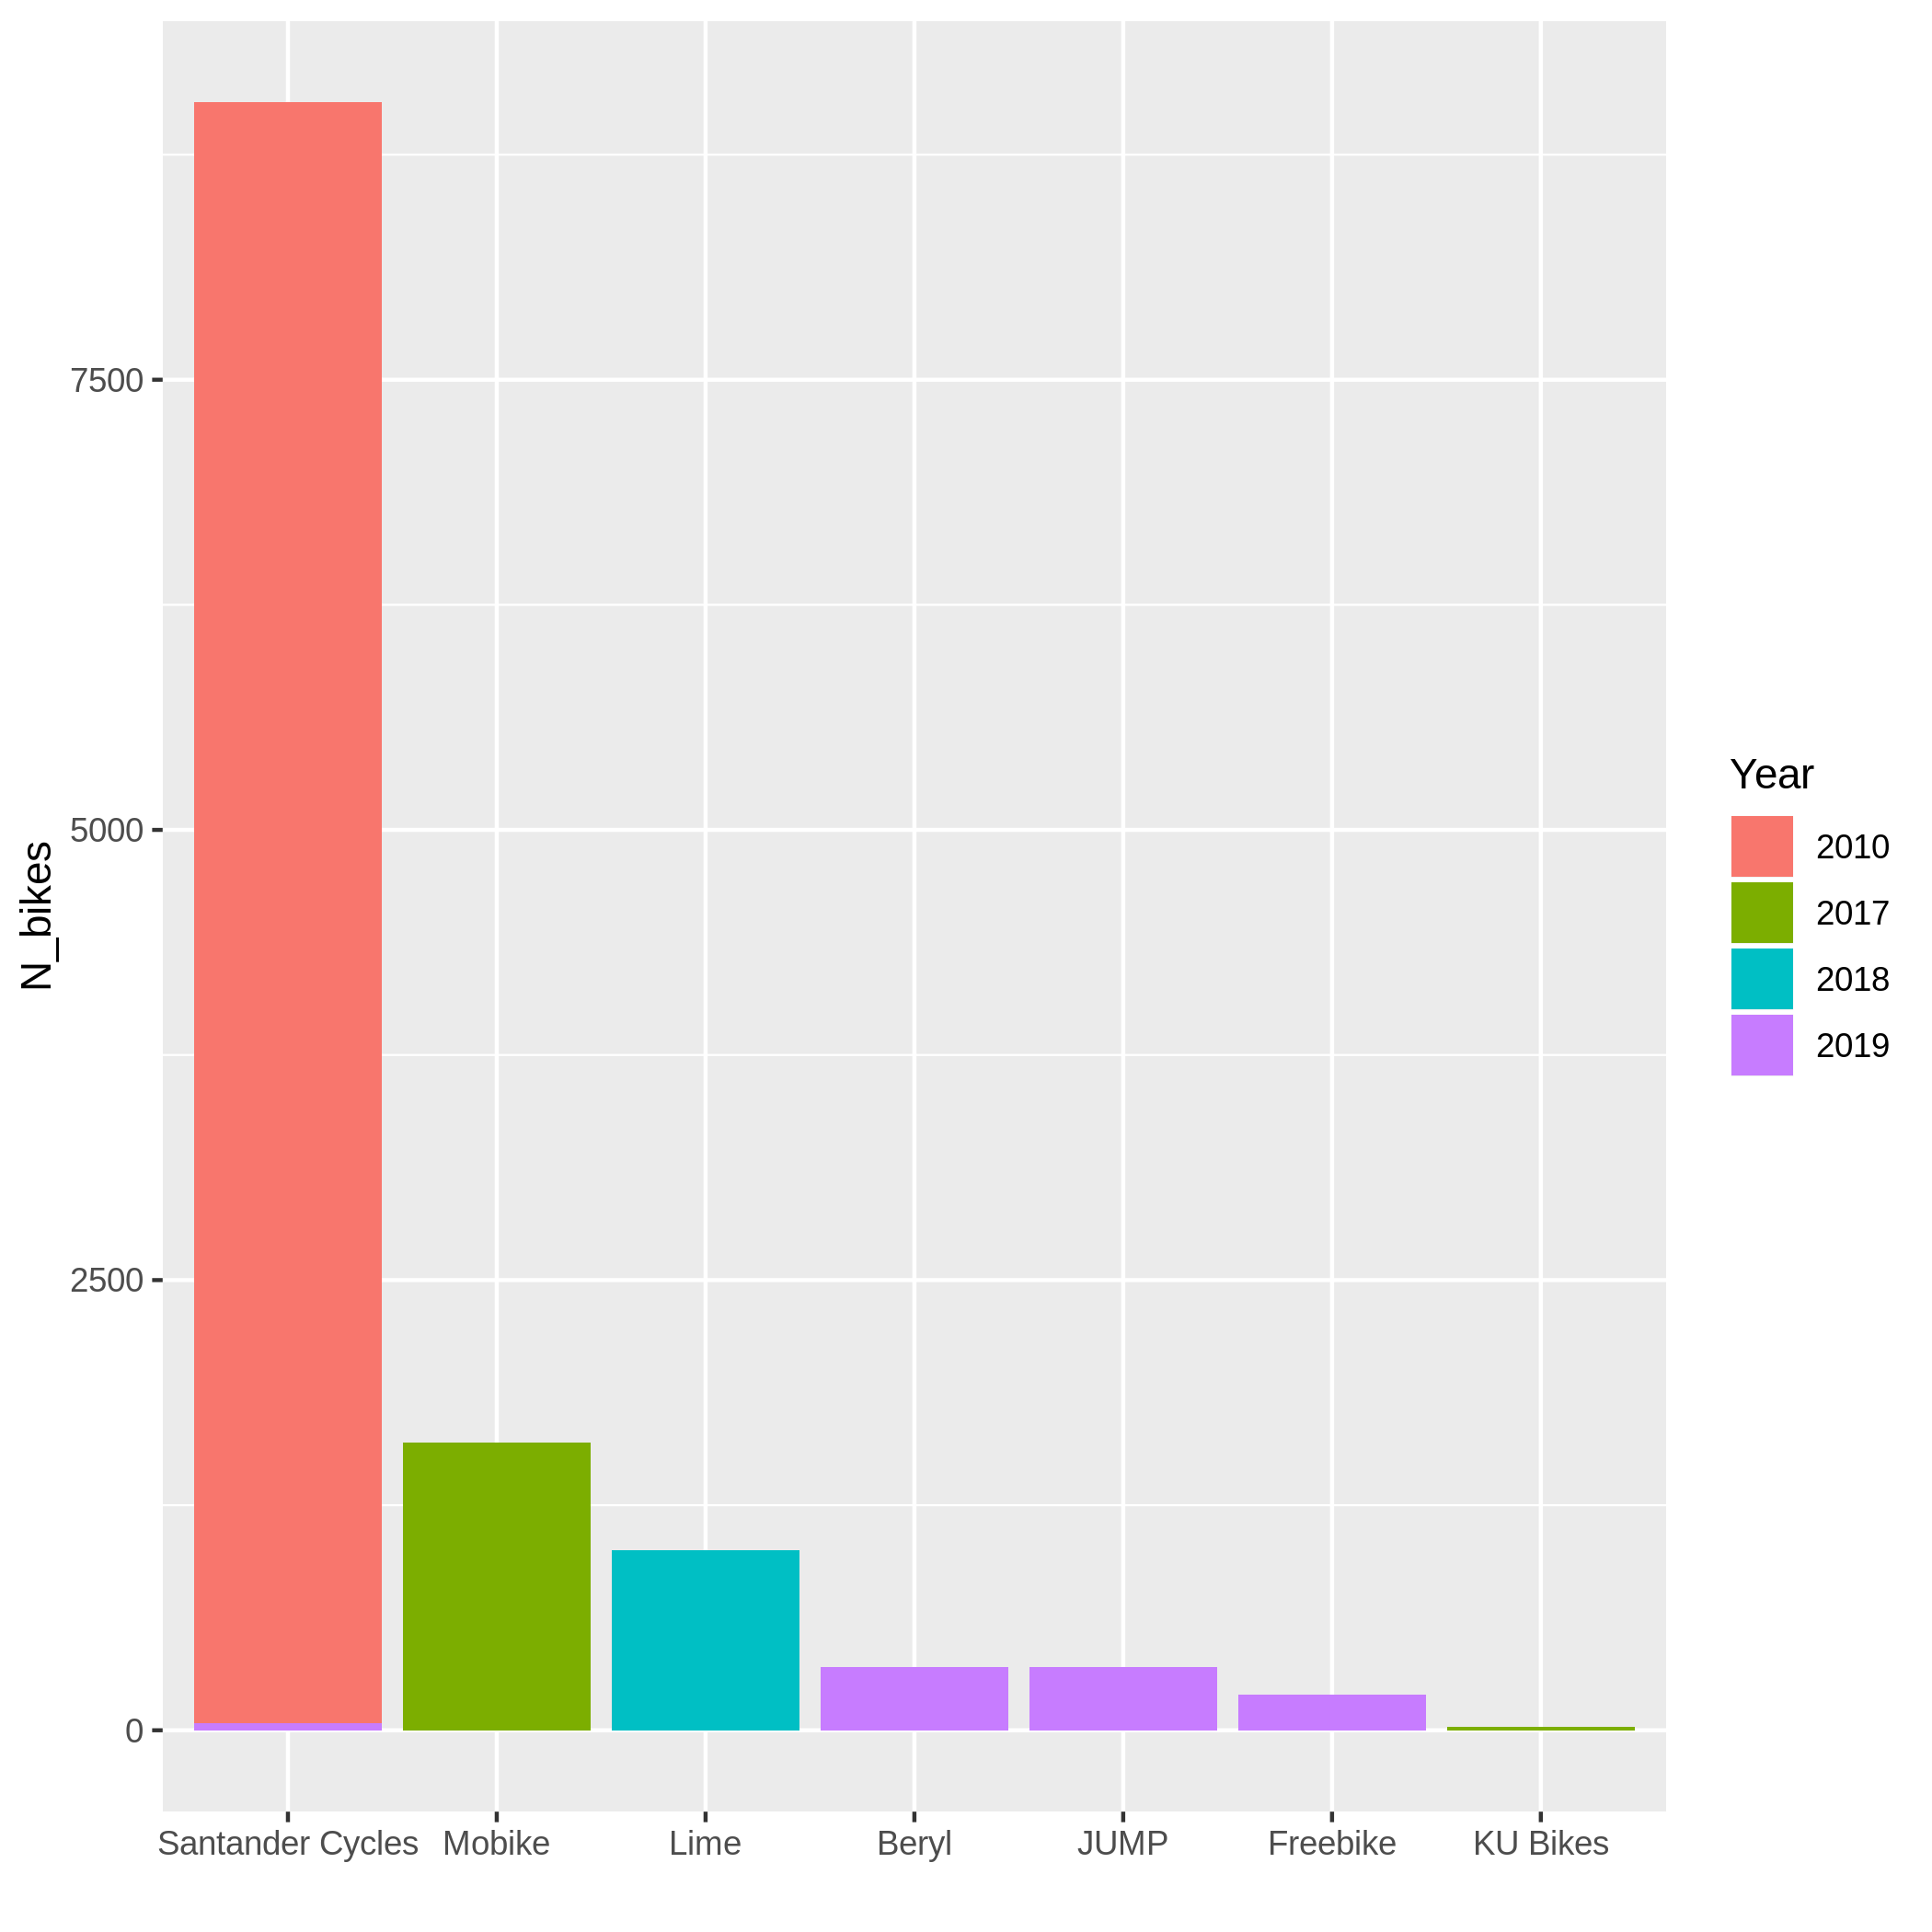
\includegraphics[width=0.7\linewidth]{figures/london-bike-hire-players} 

}

\caption{A summary of bishare schemes operating in London. Bar height proportional to number of bikes and coloured according to the year in which the scheme was introduced.}\label{fig:cycle-hire-players}
\end{figure}

There has been continued growth in usage of the scheme, as illustrated in Figure \ref{fig:cycle-hire-chart-daily}.
The main features of the graph, which runs from the 30\textsuperscript{th} July 2010 to the 30\textsuperscript{th} September 2019, correspond to events in the history of the LCHS, including:

\begin{itemize}
\tightlist
\item
  LCHS launch in late July 2010, initially with 315 docking stations and 5,000 bikes.
\item
  Expansion in March 2012 to 8,000 bikes and additional 570 stations, reflected in the rapid growth in early 2012 shown in Figure \ref{fig:cycle-hire-chart-daily}.
\item
  Expansion in December 2013 West and Southwest
  corresponding with a step change in the annual average number of hires after 2014.
\end{itemize}

\begin{figure}

{\centering 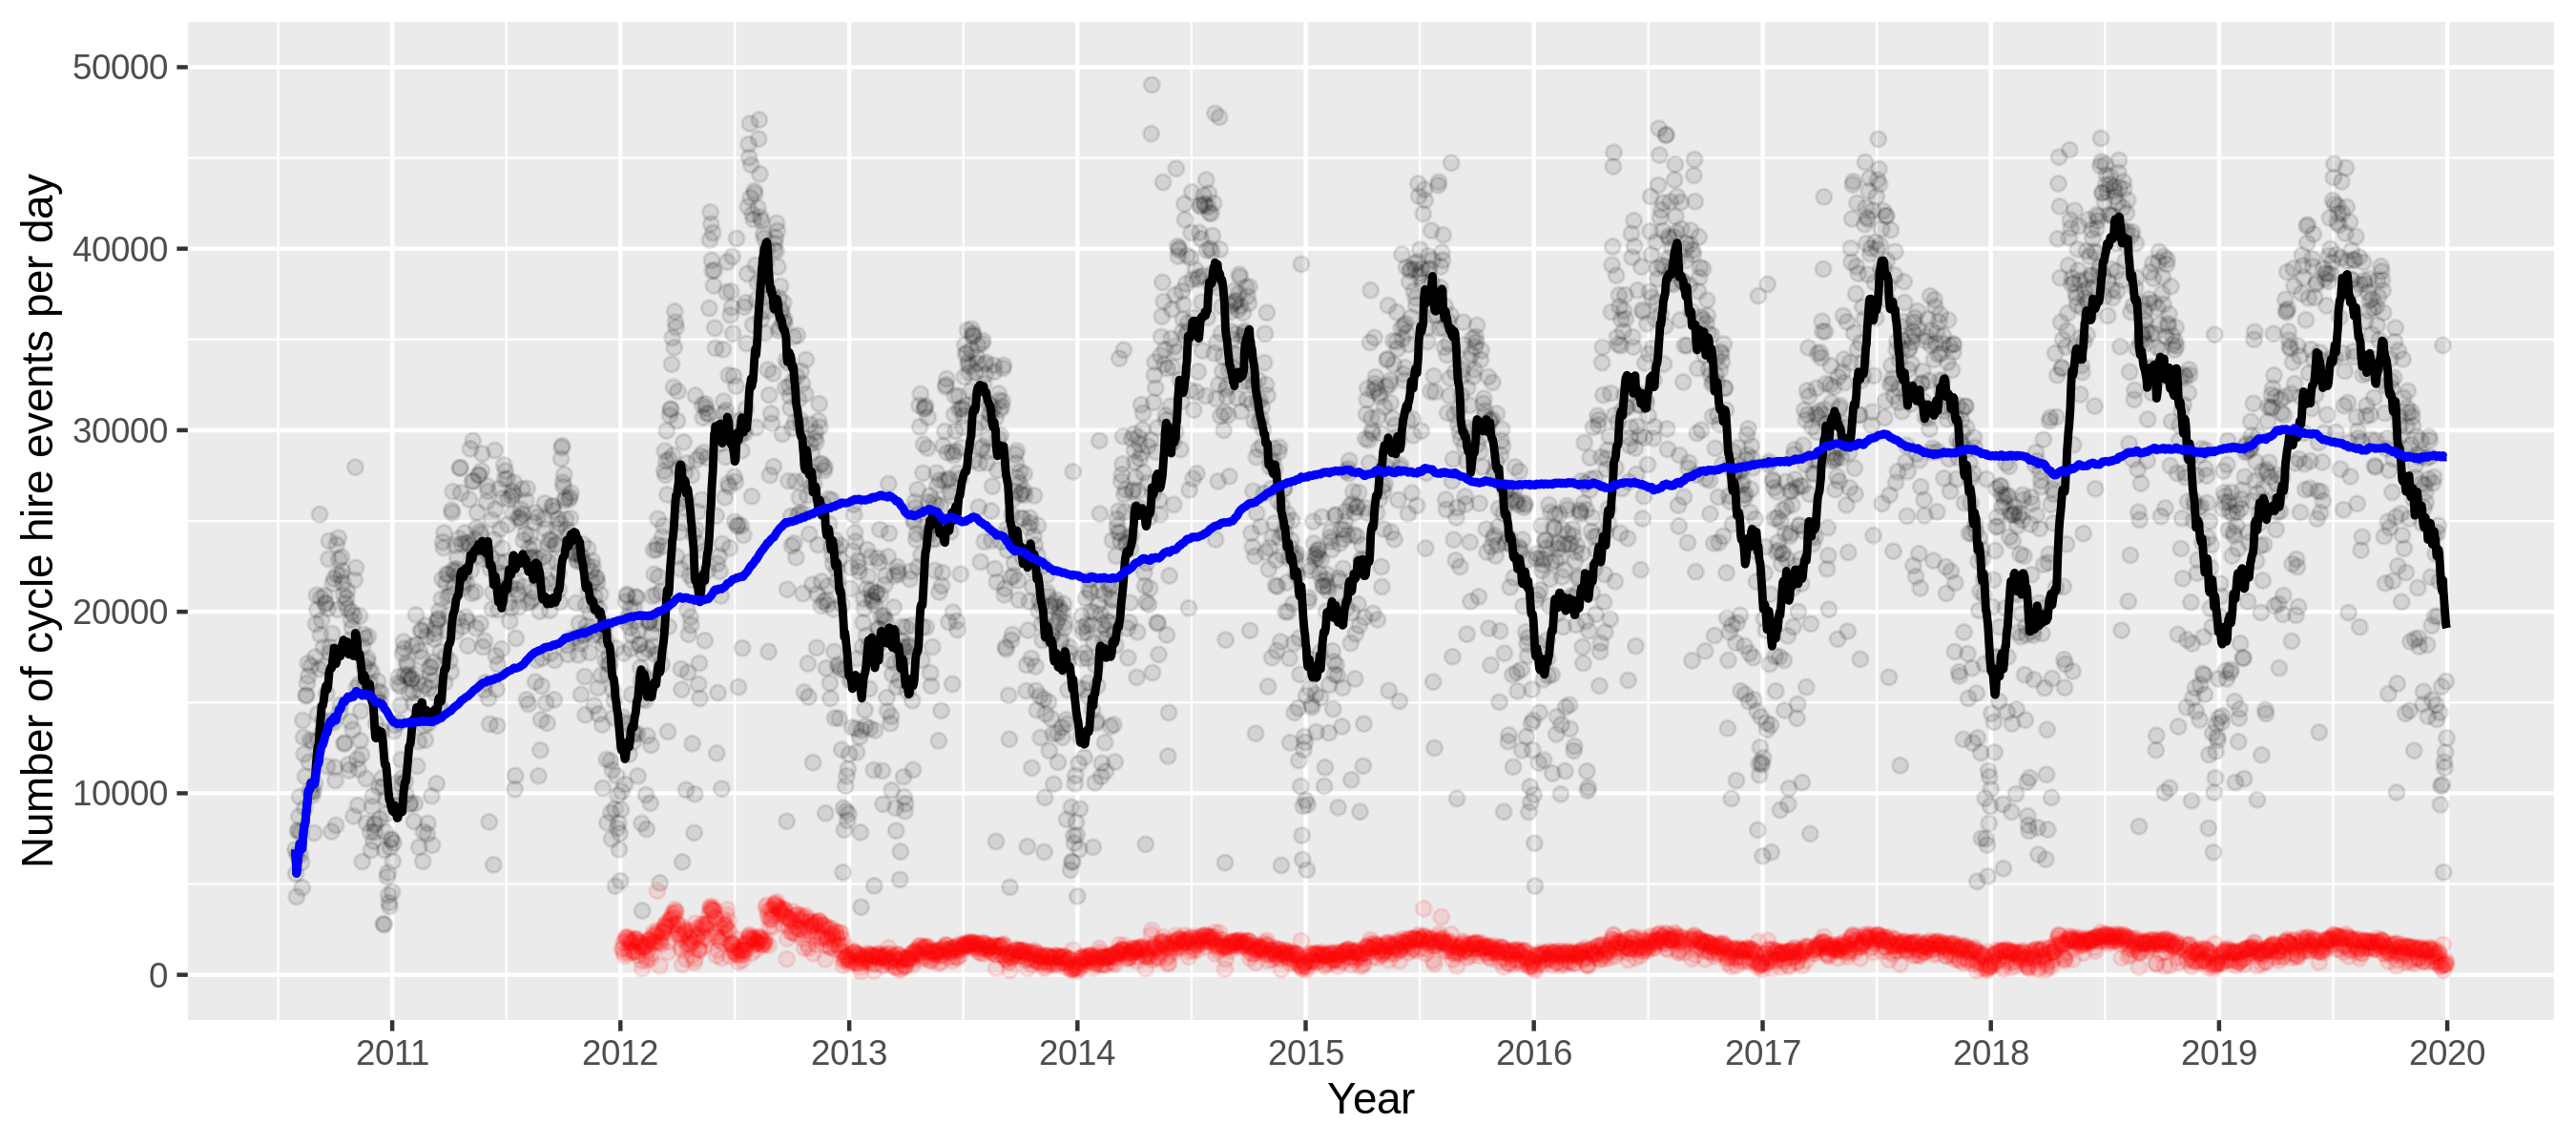
\includegraphics[width=0.7\linewidth]{figures/cycle-hire-chart-daily} 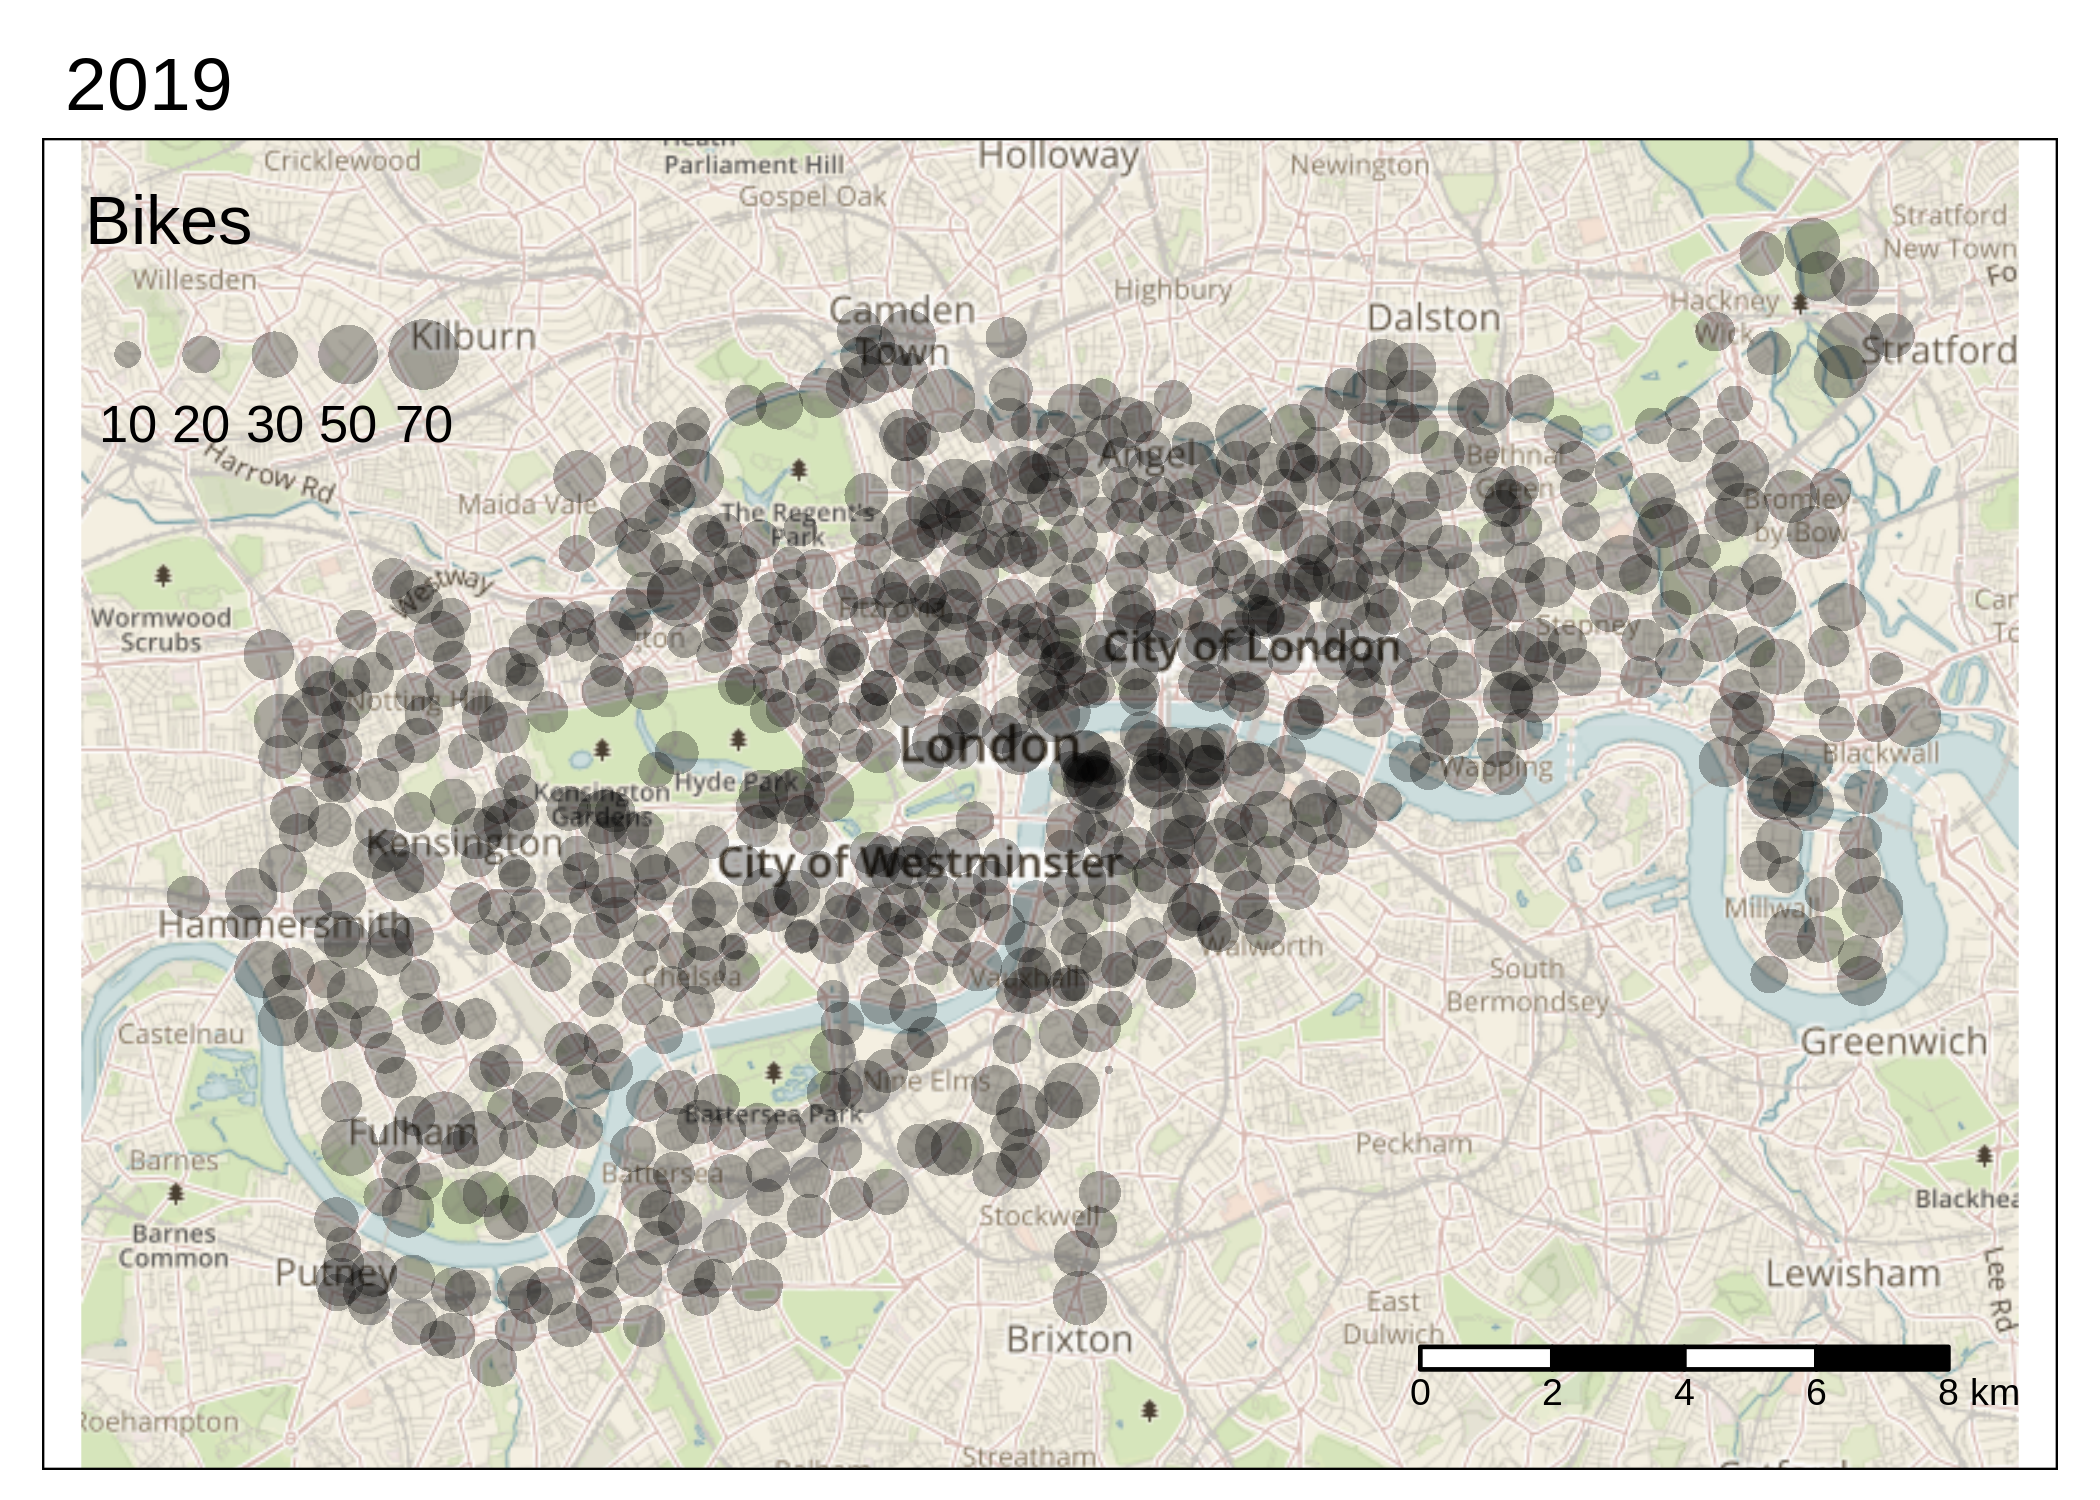
\includegraphics[width=0.7\linewidth]{figures/overview-2019} 

}

\caption{Top: Number of cycles hired per day across the London Cycle Hire Scheme, with TfL daily totals in blue and the totals from the individual trip records in black, translucent dots representing daily counts, the solid blue line representing the monthly (30 day) rolling average and dashed blue line representing the yearly rolling average. Bottom: the extent of the scheme in 2019 (see https://i.imgur.com/1rAfJgZ.gif for an animated version of the map).}\label{fig:cycle-hire-chart-daily}
\end{figure}

What was not stated in such policy documents was precisely which social groups were expected to make greatest use of the scheme.
Delivered as part of a package to ``help `normalise' the use of the bicycle as a transport mode in all situations and at any time, from commuting for work to a night out'' (Greater London Authority 2010), the LCHS was introduced at a time of massive investment in cycling.
The LCHS has continued to attract investment alongside funding for prominent schemes including Cycle Superhighways,
numerous dedicated cycle lanes,
quietways
and `mini Holland' residential interventions.
Despite cycle hire schemes being perceived as disproportionately benefiting privileged groups, there is some evidence to suggest that the LCHS has indeed helped to normalise cycling.
Goodman, Green, and Woodcock (2014) found that the scheme has a higher proportion of women than those cycling in London overall (32\% vs.~23\%), and mentions data from the London Travel Demand Survey (LTDS) showing that low income groups tend make more journeys by foot and bus than underground, implying huge potential for bikeshare in low income areas.

The Santander Cycles customer survey (TNS 2017), the sixth wave conducted since 2012, reveals that in 2017 the LCHS was primarily used by those who were male, young, white, and full-time workers.
Analysis by Morton (2018) highlighted the importance of understanding the socio-demographic make-up of users, using a market segmentation approach to support decision-making.
It was found that satisfaction with the scheme varied by market segment, with the `Low Frequenters' segment particularly sensitive to prices.
Regarding income, there were significant differences between casual users (which in 2017 represented 41\% of all users) and member users. While casual users were from all income levels in similar proportions (except for a small greater proportion of those between £20k-£40k), members over-indexed amongst the high income ranges (see figure 4).

\begin{figure}

{\centering 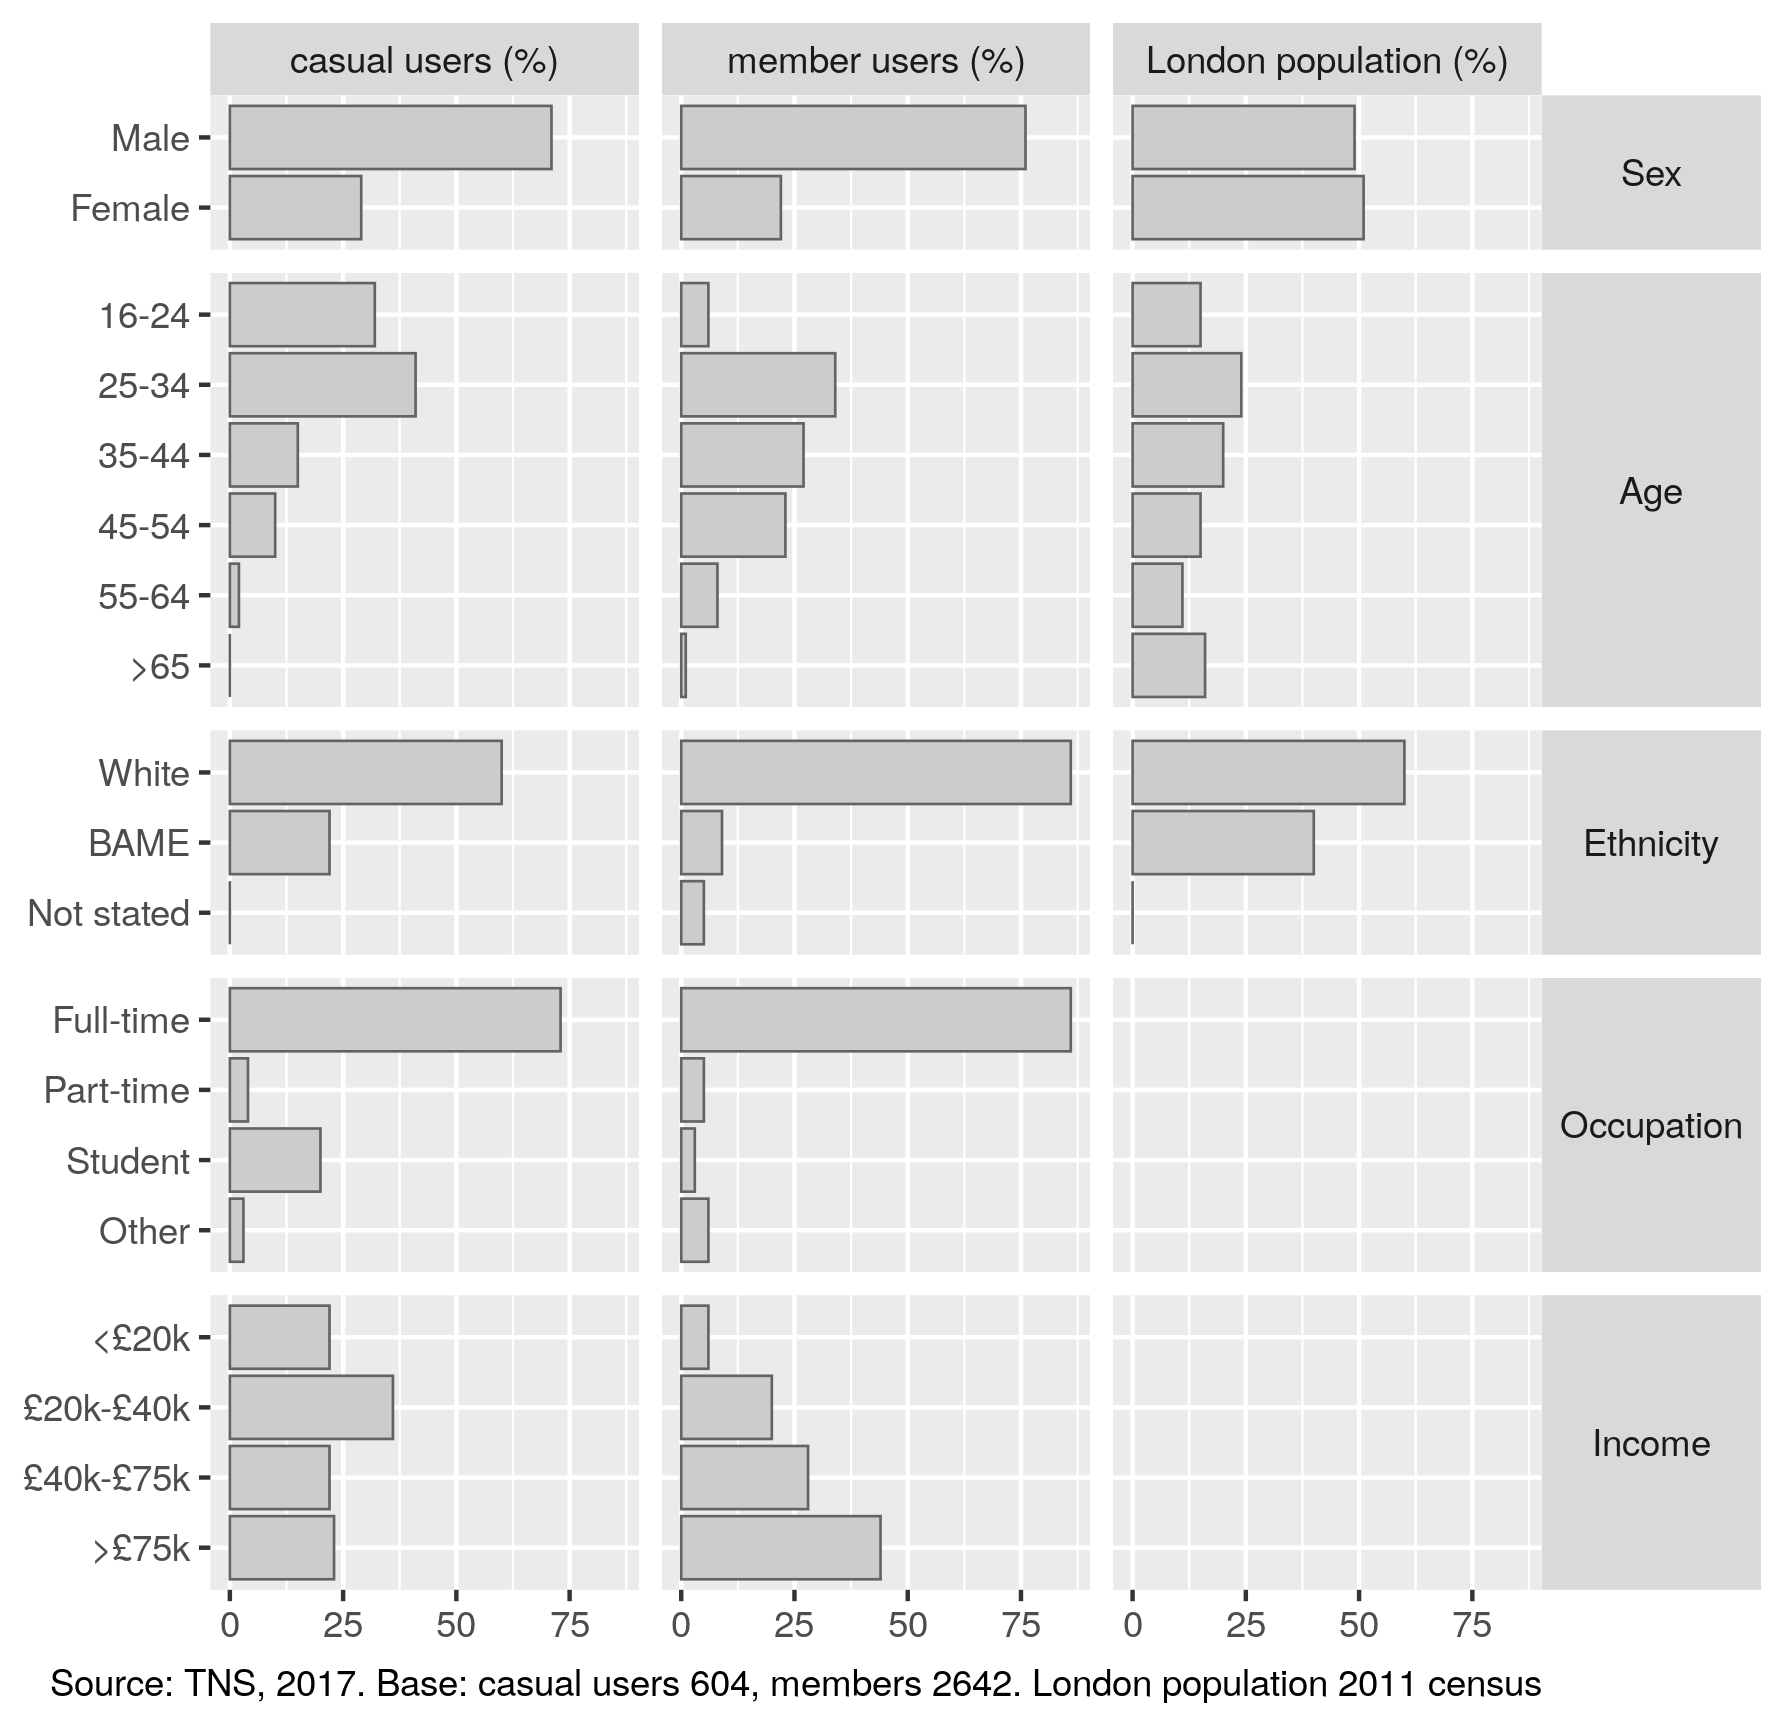
\includegraphics[width=0.7\linewidth]{figures/profile_users_lchs} 

}

\caption{Profile of the casual users and members of the LCHS}\label{fig:profile-users-lchs}
\end{figure}

A question that has not yet been addressed, however, is has the LCHS \emph{become more equal} over time?
Of course, this is a broad and to some extent subjective question because there are many ways to define `equal'.
For the purposes of this study, we will focus on spatial inequalities and focus on income inequalities, using relative levels of use between small areas (Output Areas, with around 100 households each) with high and low income levels as a proxy for equity (limitations of this methodology are discussed in the penultimate section).
The research questions are, since the LCHS scheme was expanded in 2014:

\begin{itemize}
\tightlist
\item
  Has the geographic distribution of docking stations and usage become more equal?
\item
  Has the uptake of use at docking stations in low income areas increased at a greater rate than for the scheme overall?
\end{itemize}

\hypertarget{data-and-methods}{%
\section{Data and methods}\label{data-and-methods}}

We used the open source statistical environment R (R Core Team 2020) for data processing and analysis, making use of packages such as \textbf{sf} and \textbf{ggplot2} for geographic analysis and visualisation respectively (Pebesma 2018; Wickham 2016).
To ensure reproducibility and encourage others to build on the work we have done, by saving time spent on data cleaning, the code underlying the analysis presented in this paper has been made freely available for others to learn from and use (see \href{https://github.com}{github.com/to-be-confirmed}).
A detailed account of the input datasets and methods used to characterise shifting trip patterns are provided below.

{[}Note: this repository will be made available on publication.{]}

\hypertarget{trip-and-station-datasets}{%
\subsection{Trip and station datasets}\label{trip-and-station-datasets}}

Data on docking stations was provided by the Consumer Data Research Centre (\href{https://data.cdrc.ac.uk/product/ffc94eb2-baf0-46f9-bf7d-5e8dd424b95d?accesslevel=open\&q=\&sort=title_string+asc}{data.cdrc.ac.uk}).
This was made available in a `.csv' file containing 1,130 rows with 19 variables including docking station ID, name, location coordinates and its opening date.
The other key dataset used in this study was Origin-Destination (OD) trip data, published by \href{https://cycling.data.tfl.gov.uk}{Transport for London} and accessed via the \href{https://github.com/ropensci/bikedata}{bikedata} R package (Padgham and Ellison 2017).
Both datasets were linked via a docking station ID.
In the \emph{trips} table, the origin and destination docking station and corresponding timestamps is recorded.
The \emph{docking station} table contains IDs, names and geographic coordinates for each docking station.
A script was developed to clean the raw data, remove duplicate trips and ensure that records omitted from the bikedata package (version \texttt{0.2.3}) were included in the analysis.
In total 73.4 million trips, with known start and end points, were recorded from January 2012 until the end of December 2019 (see Figure \ref{fig:cycle-hire-chart-daily}).

\hypertarget{socio-demographic-data}{%
\subsection{Socio-demographic data}\label{socio-demographic-data}}

To characterise the shifting spatial inequalities in the provision of bikeshare infrastructure in London, we joined residential zone data (at the LSOA level) to each docking station.
First we defined the study area as a polygon resulting from a 500 m buffer around the `concave hull' of the docking stations.
To estimate `residential populations' who live in close proximity to docking stations, we developed a three-stage methodology involving: 1) estimating the average number of inhabitants per building, based on the smallest `Output Area' population estimates and building footprint data from OpenStreetMap; 2) identifying residential buildings within a threshold distance (150, 200 and 300 m buffer distances were tested) of docking stations; and 3) assigning the total estimated population in these buildings to their associated docking station (see Figure \ref{fig:bikeshare-resi-buildings}).
Considering the density of docking stations and access to alternative transport options such as bus stops, we opted for the smallest of the buffer distances tested for the results presented.
The use of different buffer distances did not change the direction of the results or conclusions drawn from them (see Discussion).

\begin{figure}

{\centering 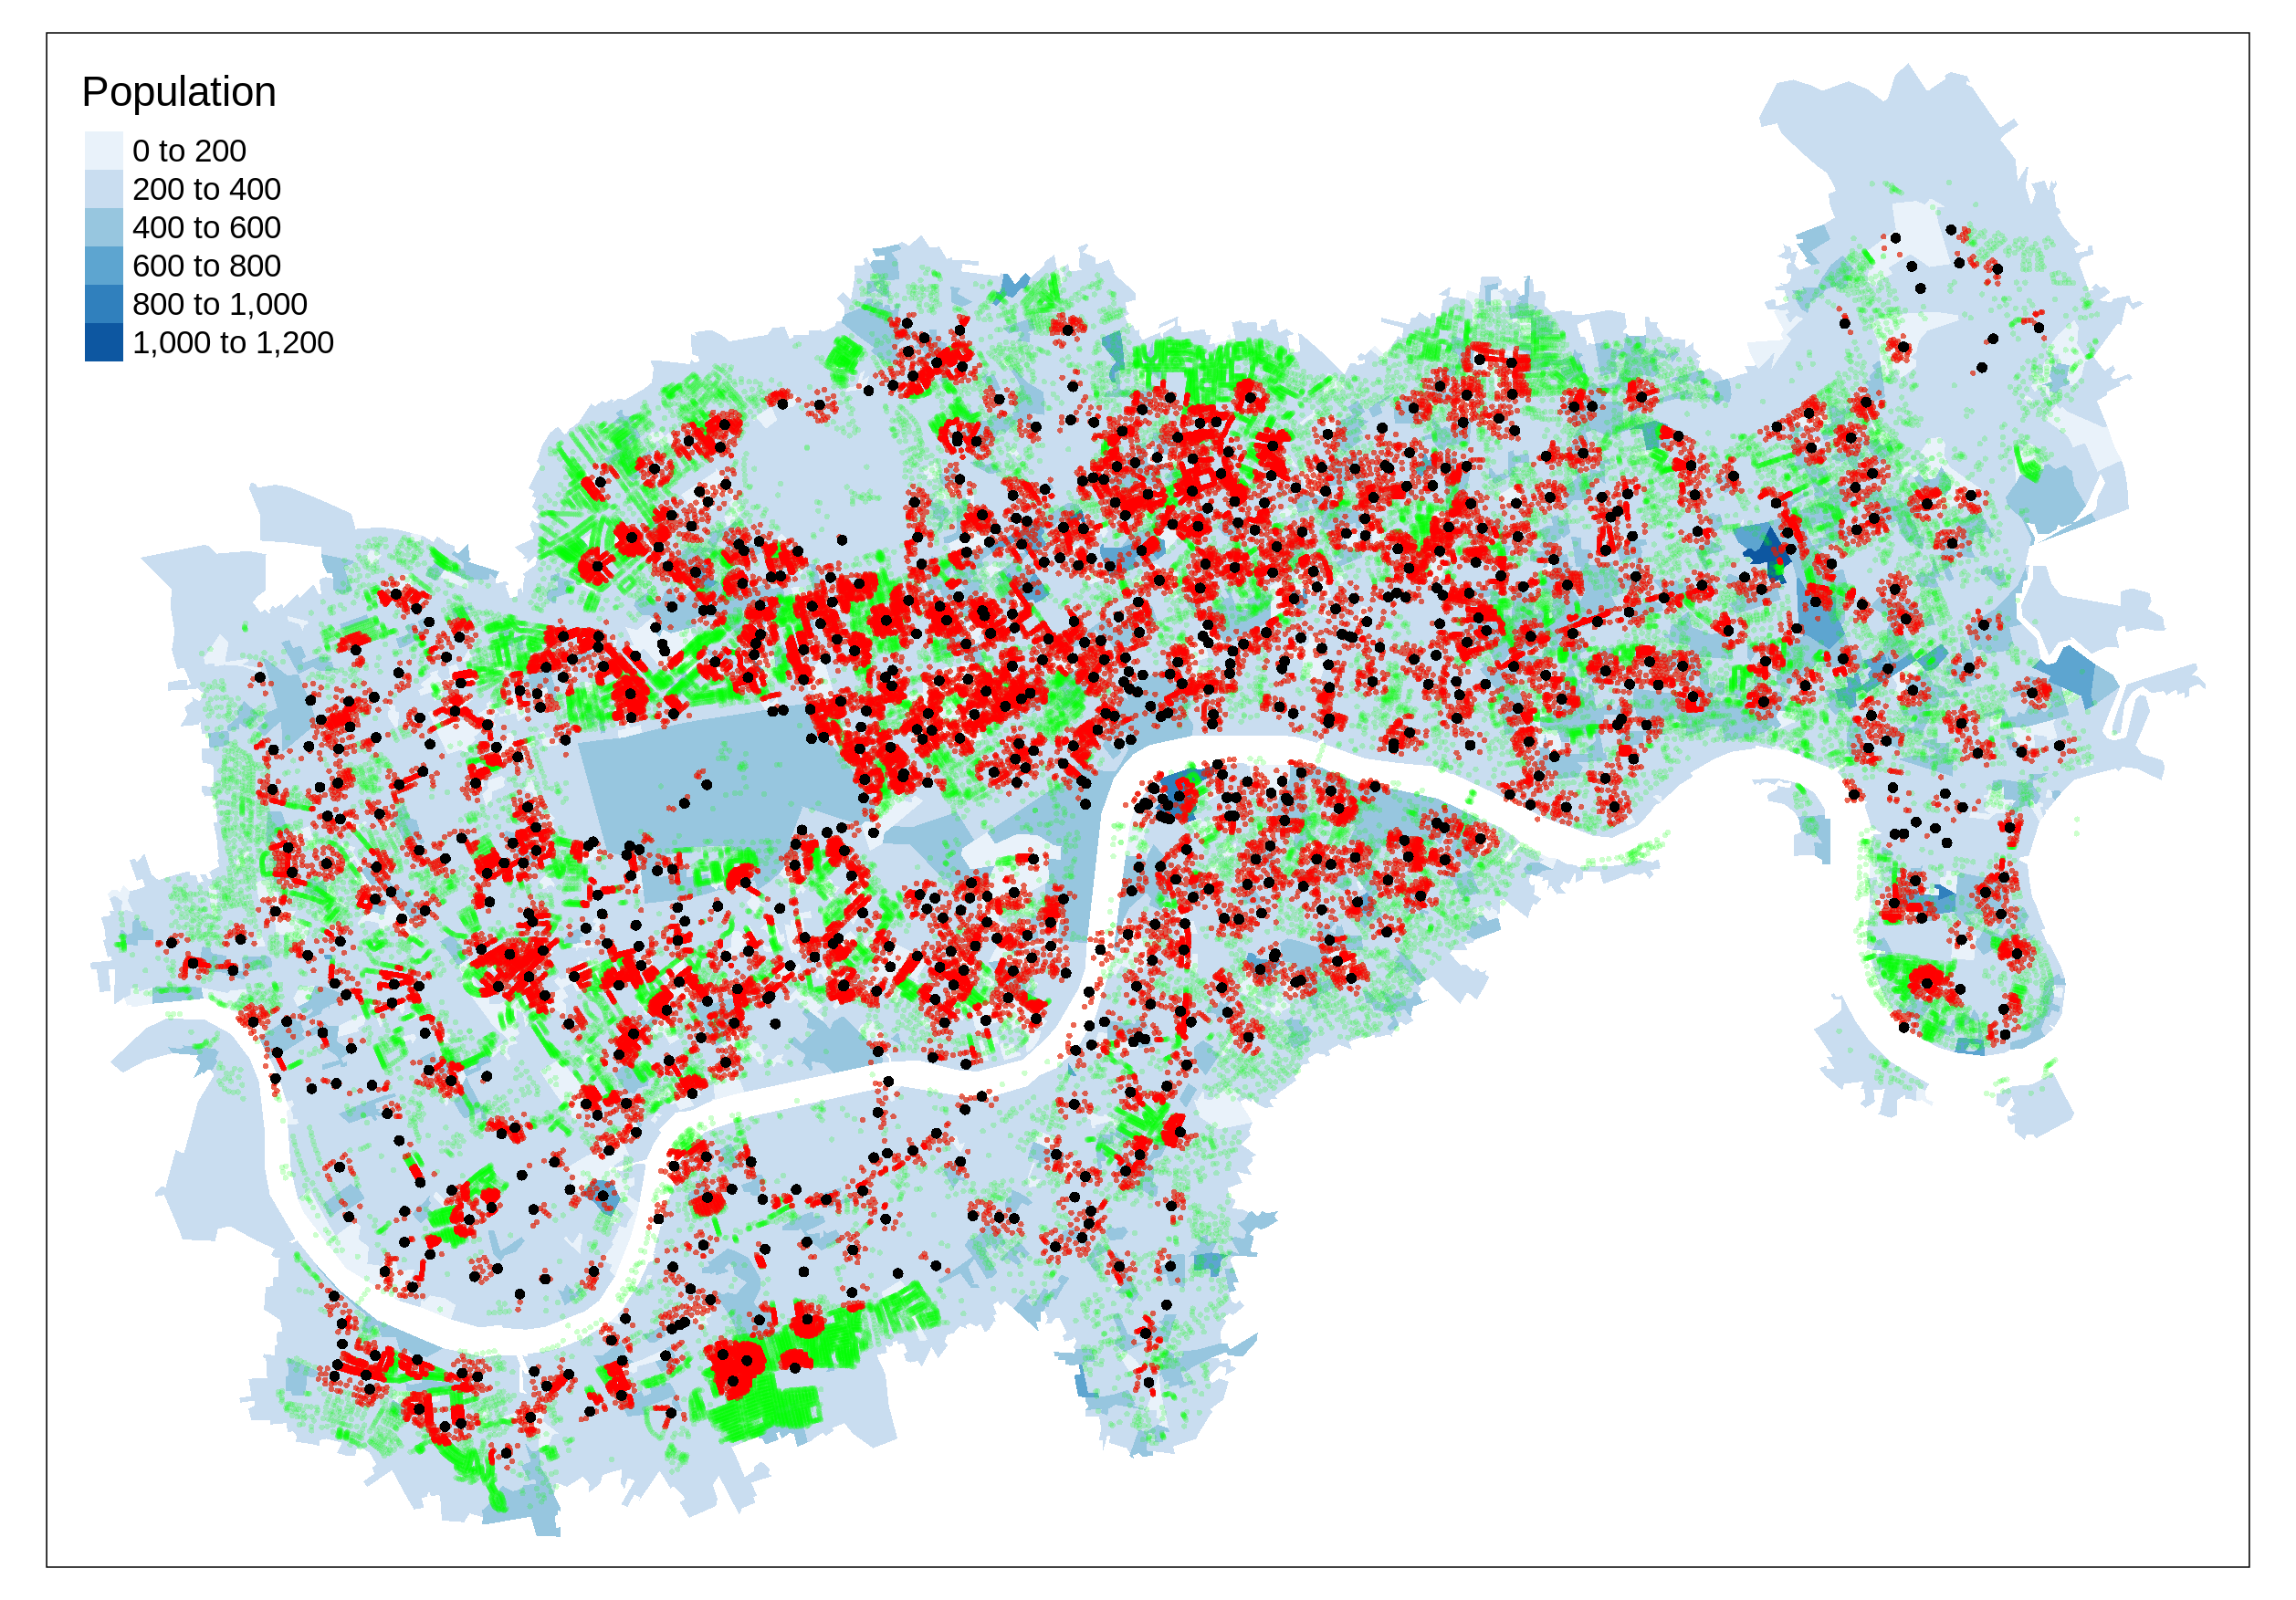
\includegraphics[width=0.7\linewidth]{figures/bikeshare-resi-buildings} 

}

\caption{Method for estimating the residential population with access to docking stations within 150m. Blue shade represents the population in each Output Area, buildings are in green and buildings near docking stations are in red.}\label{fig:bikeshare-resi-buildings}
\end{figure}

Official population data from the 2011 Census were collected at Output Area and 2015 estimates of the Index of Multiple Deprivation and income deciles at the LSOA level.\footnote{See \url{https://data.cdrc.ac.uk/dataset/4d3a8738-38af-401c-8070-6be5d85b2f5e}}

\hypertarget{inferring-residential-trips}{%
\subsection{Inferring residential trips}\label{inferring-residential-trips}}

Since users' home locations and trip purpose are not stored in the OD data, it is impossible to know which trips were made by local residents and which were not.
However, it is possible to infer residential usage from trip patterns.
The daily flow of cycle hire scheme usage shows a clear pattern, with the majority of `home station trips' (in which bikes are rented near the user's home) happening in the morning peak (which we define as 06:00 to 10:00).
The comparison between morning and afternoon usage patterns highlights the reasons for this emphasis: in the afternoon peak (16:00 to 20:00) many trips represent people renting cycles in the centre for the return leg of their journey and many more tourist and leisure trips are taken by non-residents during this time (see Figure \ref{fig:map-am-pm-peaks}).

By taking AM and PM peak subsets from the full dataset, and calculating the number of trips per year per docking station and associated IMD scores (income component) we could generate results estimating both the overall levels of usage per resident per year by income levels of the areas in which docking stations are located, and the relative levels of growth in relatively high and low income areas.
These results are presented in the next section.

\begin{figure}

{\centering 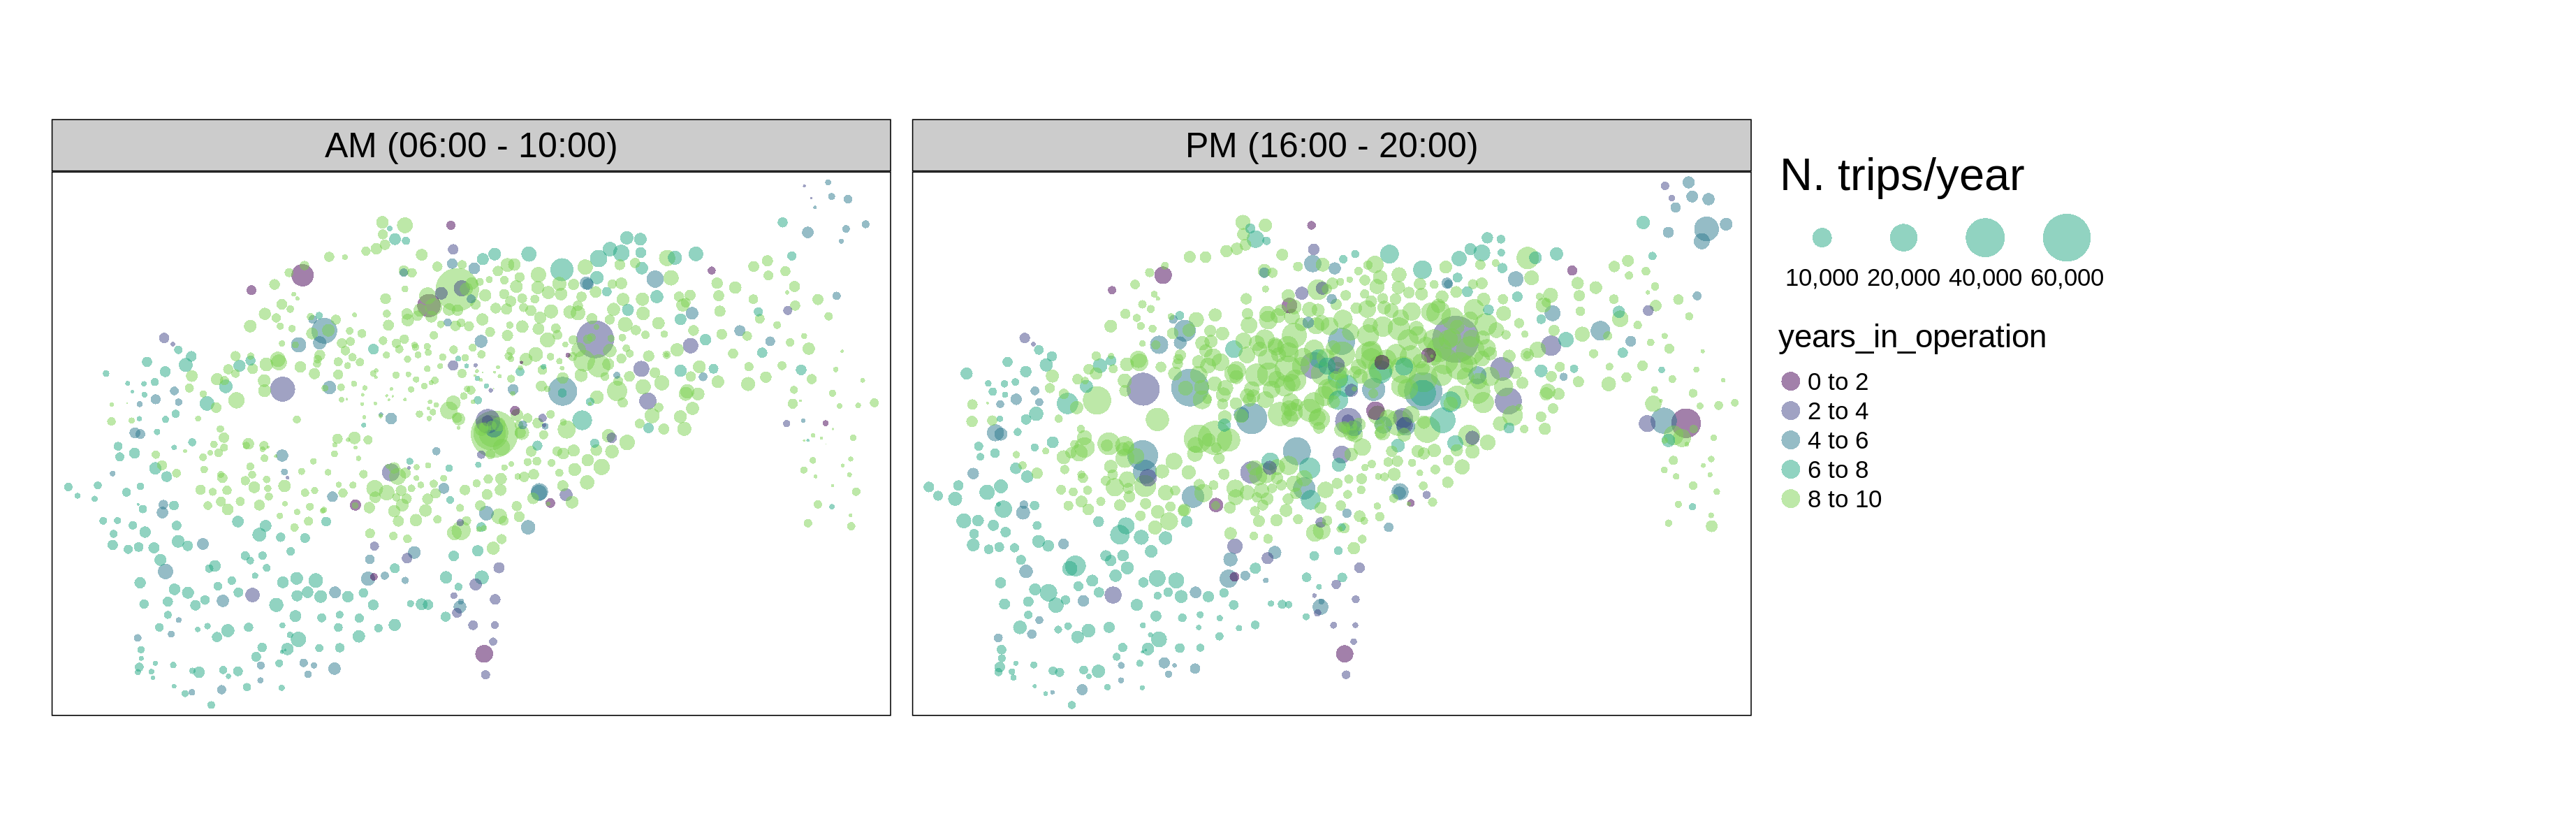
\includegraphics[width=1\linewidth]{figures/map-am-pm-peaks} 

}

\caption{Spatial distribution of cycle hire points of origin during the morning and afternoon peaks}\label{fig:map-am-pm-peaks}
\end{figure}

\hypertarget{results}{%
\section{Results}\label{results}}

\hypertarget{change-in-areas-served-by-docking-stations}{%
\subsection{Change in areas served by docking stations}\label{change-in-areas-served-by-docking-stations}}

The evolving spatial distribution of the LCHS is illustrated in Figure \ref{fig:facet-map} (top), which shows that its expansion into residential areas corresponded with a shift towards lower income communities.
The map illustrates that the scheme has not expanded uniformly, with Phase 2 expanding into Tower Hamlets, to the East of the scheme and Phase 3 into areas south of the river such as Wandsworth and Clapham Junction in Southwest central London.
It seems that particular areas such as the area to the east of Hackney in the far north-east of the plot, and the cluster of docking stations going to Brixton in the central south region of the map, were targeted deliberately.
It is interesting to note that these demographically diverse geographic outliers were selected instead of more geographically central areas such as Bermondsey (on the South bank of the River Thames to the East), leading to the `why the gap' campaign for the scheme to be expanded into this part of the city.\footnote{See \href{http://whythegap.london}{whythegap.london} for the campaign for ``Cycle Hire Scheme for Rotherhithe and Bermondsey'', which contains quotes from many people on the importance of expanding the scheme, including London Mayor Sadiq Kahn who is quoted as saying:
  ``There are lots of anomalies in that cycle hire scheme. We are going to explore them.''}

\begin{figure}

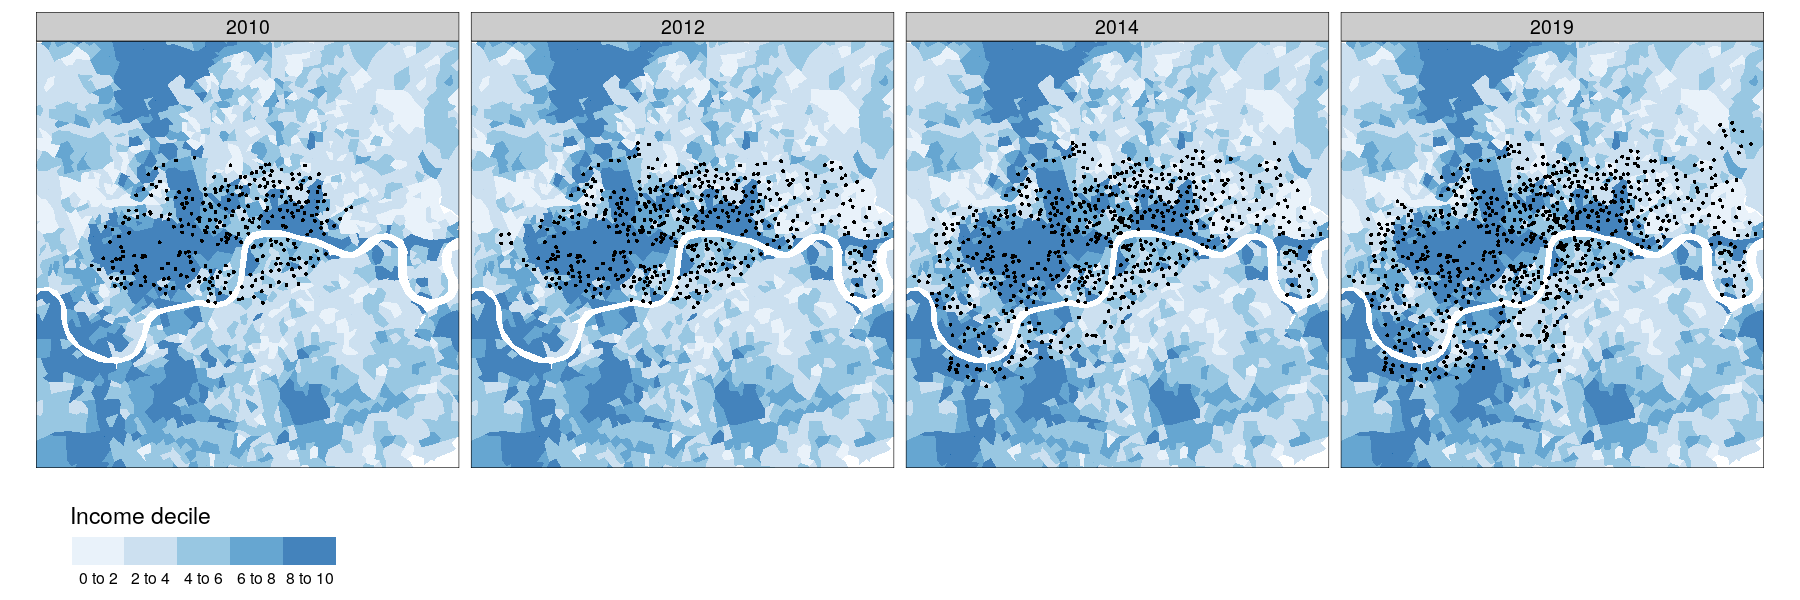
\includegraphics[width=1\linewidth]{figures/facet-imd} 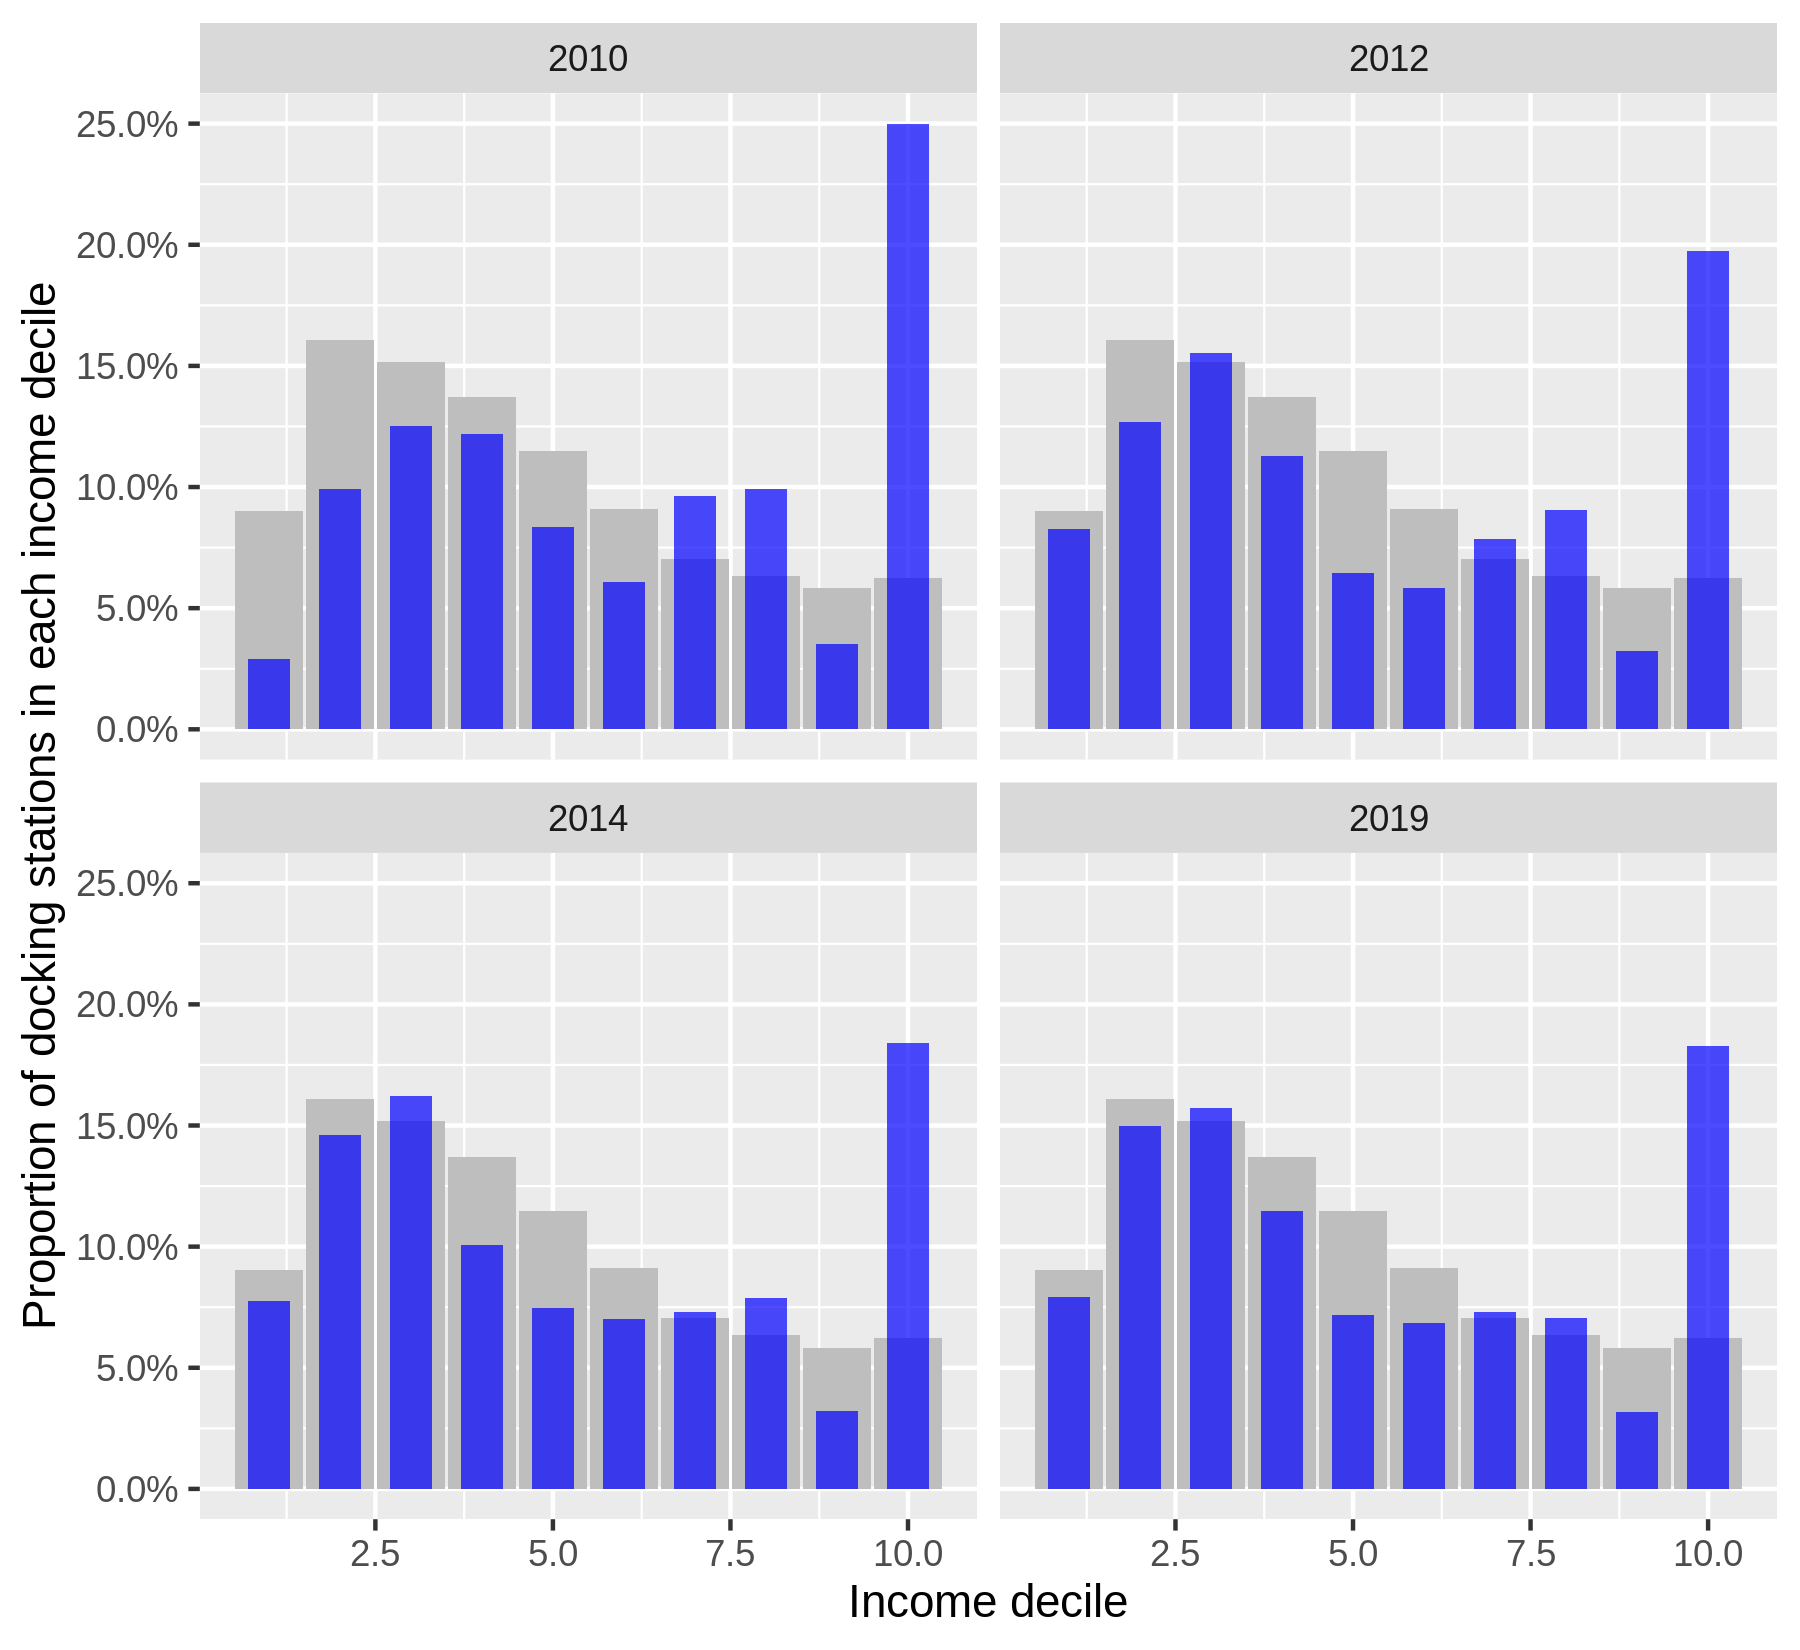
\includegraphics[width=1\linewidth]{figures/stations-imd-facet-4-grey} \hfill{}

\caption{Changes in the spatial and social distribution of docking stations over time, 2010-2019, showing four stages of expansion. Zone colour represents income decile, with 1 (white) representing the lowest income areas and 10 represents (blue) wealthy areas (top). The percentage of docking station in each income decile over time (blue) overlaying a representative distribution of income deciles for London (grey) for the same years (bottom). Note: a distribution representative of national income levels would be flat.}\label{fig:facet-map}
\end{figure}

Figure \ref{fig:facet-map} (bottom) shows the percentage of docking stations associated with each income decile for each of the four years plotted in map above (2010, 2012, 2014, 2019).
This clearly shows that the provision of bikeshare opportunities in income areas has increased year-on-year, becoming more representative of London overall, in terms of income deciles of LSOA zones (the proportion of zones in each income decile is repeated in grey).
Overall, the average income decile associated with docking stations has dropped from 5.7 to 4.9 since the scheme's inception and the standard deviation has increased slightly from 2.87 income deciles to 2.94.
The question remains whether this increased provision of docking stations in low income areas also coincided with increased used in those areas?

\hypertarget{income-distribution-of-docking-station-usage}{%
\subsection{Income distribution of docking station usage}\label{income-distribution-of-docking-station-usage}}

The relationship between docking station usage and levels of income deprivation at trip origins varies by time of day.
During the morning peak trips originating in more residential areas container comparatively high income deprivation (excluding stations by major transport hubs) are more common, per local resident per year.
In the PM peak, docking stations serving low income deprivation areas have more traffic as illustrated in Figure \ref{fig:income-decile-am-pm-beeswarm}, a boxplot that shows median levels of usage for morning (top) and afternoon (bottom) rush hours (not influenced by major docking stations serving large transport hubs).
This can partly be explained by the social-spatial geography of disadvantage in London, which tends not to cluster in central places that employ many people.
In the morning peak there is a mass movement of people from residential areas containing income deprivation into the city centre for work, a pattern that reverses in the afternoon.
The spatial distribution of the morning peak origins is likely to reflect the home location of BSS users better than the evening peak.
Based on this measure, the scheme seems to be relatively inclusive, with similar median levels of usage across all income deciles except for docking stations in zones with an income decile of 4 (mid-level income deprivation) which have high levels of usage per resident person per year and docking stations in zones with an income decile of 7 (comparatively lower income deprivation), which are associated with relatively low levels of usage.
But how has usage changed over time?

\begin{figure}

{\centering 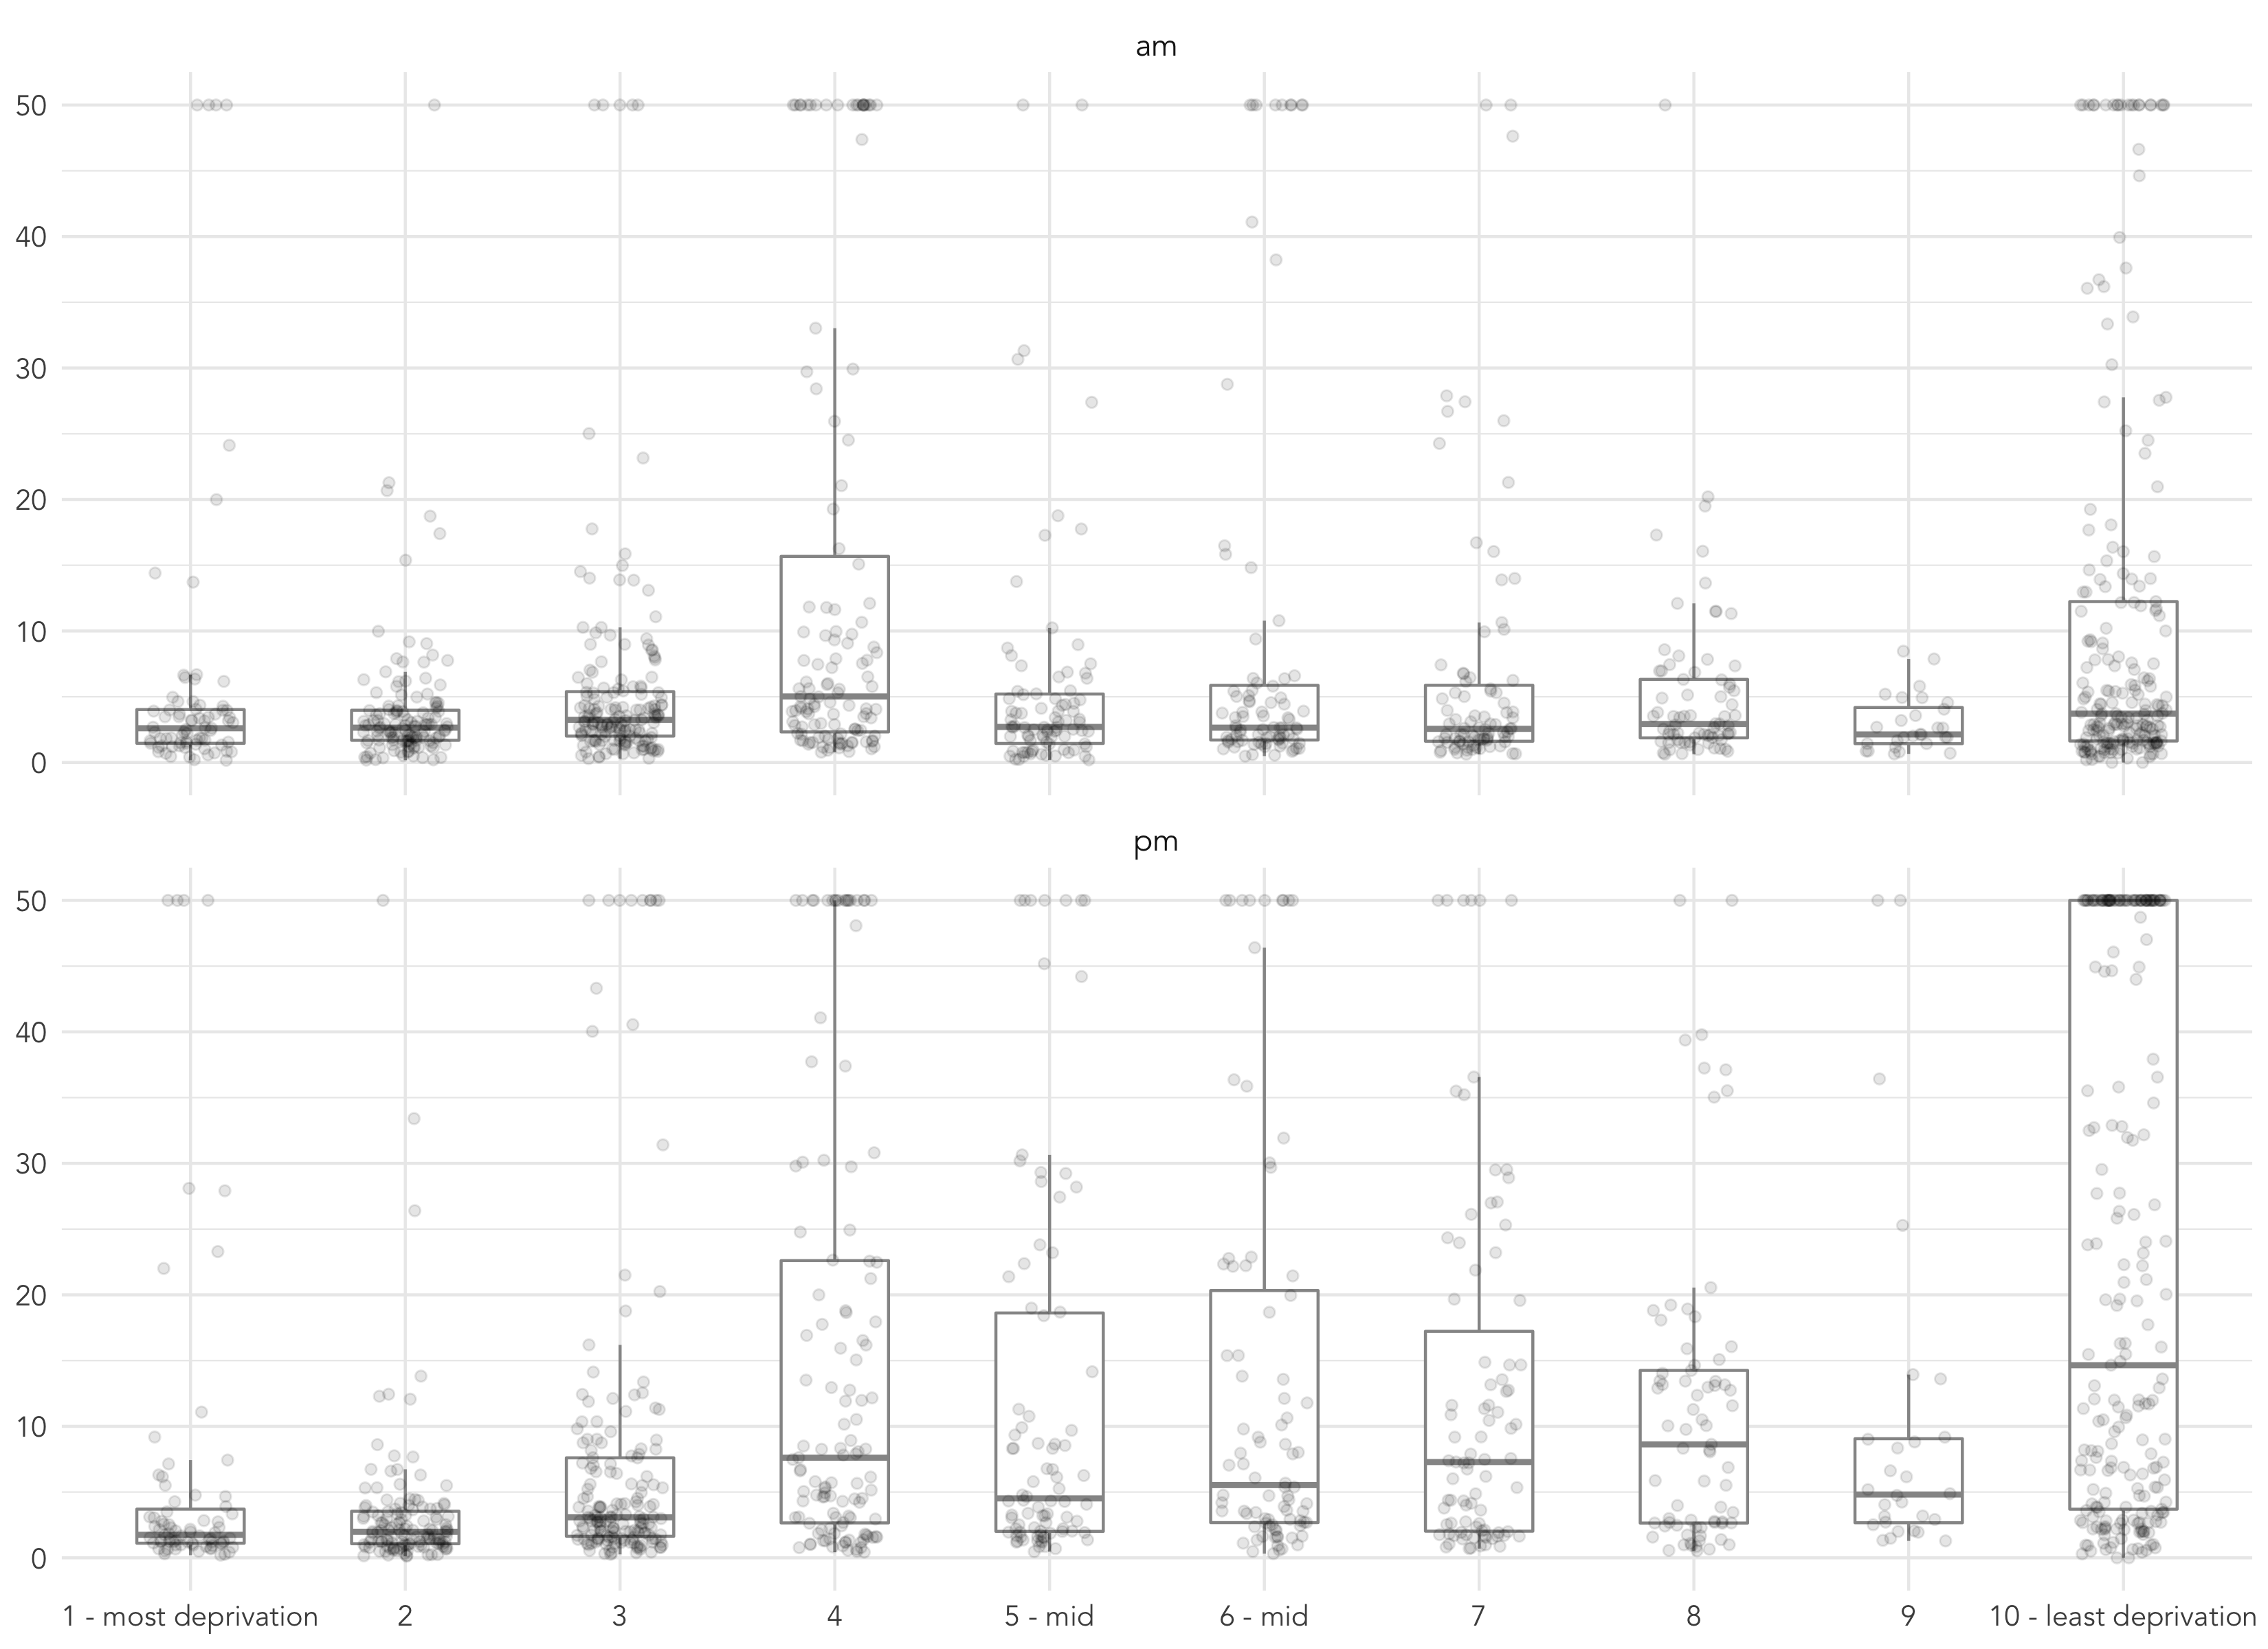
\includegraphics[width=0.7\linewidth]{figures/income-decile-am-pm-boxplot_minor} 

}

\caption{Boxplot showing docking station usage (y axis) by income decile of nearest residential areas (x axis, ordered left-to-right by high-to-low deprivation) during the morning (top panel, 06:00 to 10:00) and afternoon (bottom panel, 16:00 to 20:00) peaks. In order to clean out extreme values at hub stations, average trip counts are censored to 50}\label{fig:income-decile-am-pm-beeswarm}
\end{figure}

\hypertarget{changes-in-usage-over-time}{%
\subsection{Changes in usage over time}\label{changes-in-usage-over-time}}

Contrary to expectations, cycle hire usage does not seem to be lower in low income areas.
But is this a recent trend?
Figure \ref{fig:change-time-income} explores this by showing the number of trips starting at docking stations associated with each income decile (again with 1 and 10 being the most and least income-deprived deciles respectively) over time.
These are daily counts smoothed over a 365-day period and, in order to compare within each income decile category, a local scaling is used per income decile.
Changes in counts for all docking stations in that income decile is coloured red; the thin grey lines are counts by individual docking stations with a local scaling per docking station, again to support relative comparison.
The addition of individual-level docking station data gives an indication of how representative the overall trend (in red) is across individual docking stations. In Figure \ref{fig:change-time-boroughs} the same encoding is used, but docking stations are grouped by London borough and arranged according to their approximate spatial position. It should be noted that direct comparison of the overall and station-level trends (grey and red lines) should be treated with caution as the change in overall counts (red) is partly a function of scheme expansion -- a corollary of more docking stations in certain boroughs or income deciles is, presumably, elevated trip counts in those areas.

The patterns implied by these charts are instructive. Docking stations in central and ``prime'' London and where the scheme is typically at capacity -- Westminster and City of London and with many in income decile 10 -- show consistently high frequencies throughout the study period. There is strong pattern of increasing usage in parts of London associated with the western expansion (Hammersmith \& Fulham, Wandsworth and parts of Lambeth) and to a lesser extent eastern expansion (Tower Hamlets and parts of Hackney). Particularly striking is the consistently increasing trip frequencies in Wandsworth and also further east in Lambeth and Southwark. These boroughs containing large working populations on the edge, or outside of, ``prime'' London, have recently benefited from new cycle infrastructure -- cycle superhighways often with segregated cycle lanes, completed between 2016 and 2018. That we see large relative increases in trip frequencies for docking stations in these boroughs perhaps suggests a more utilitarian and residential usage characteristic than the dominant stereotype for the LCHS of the rail commuter making regular peak-time journeys between hub stations or the tourist making occasional leisure journeys in London's parks.

\begin{figure}

{\centering 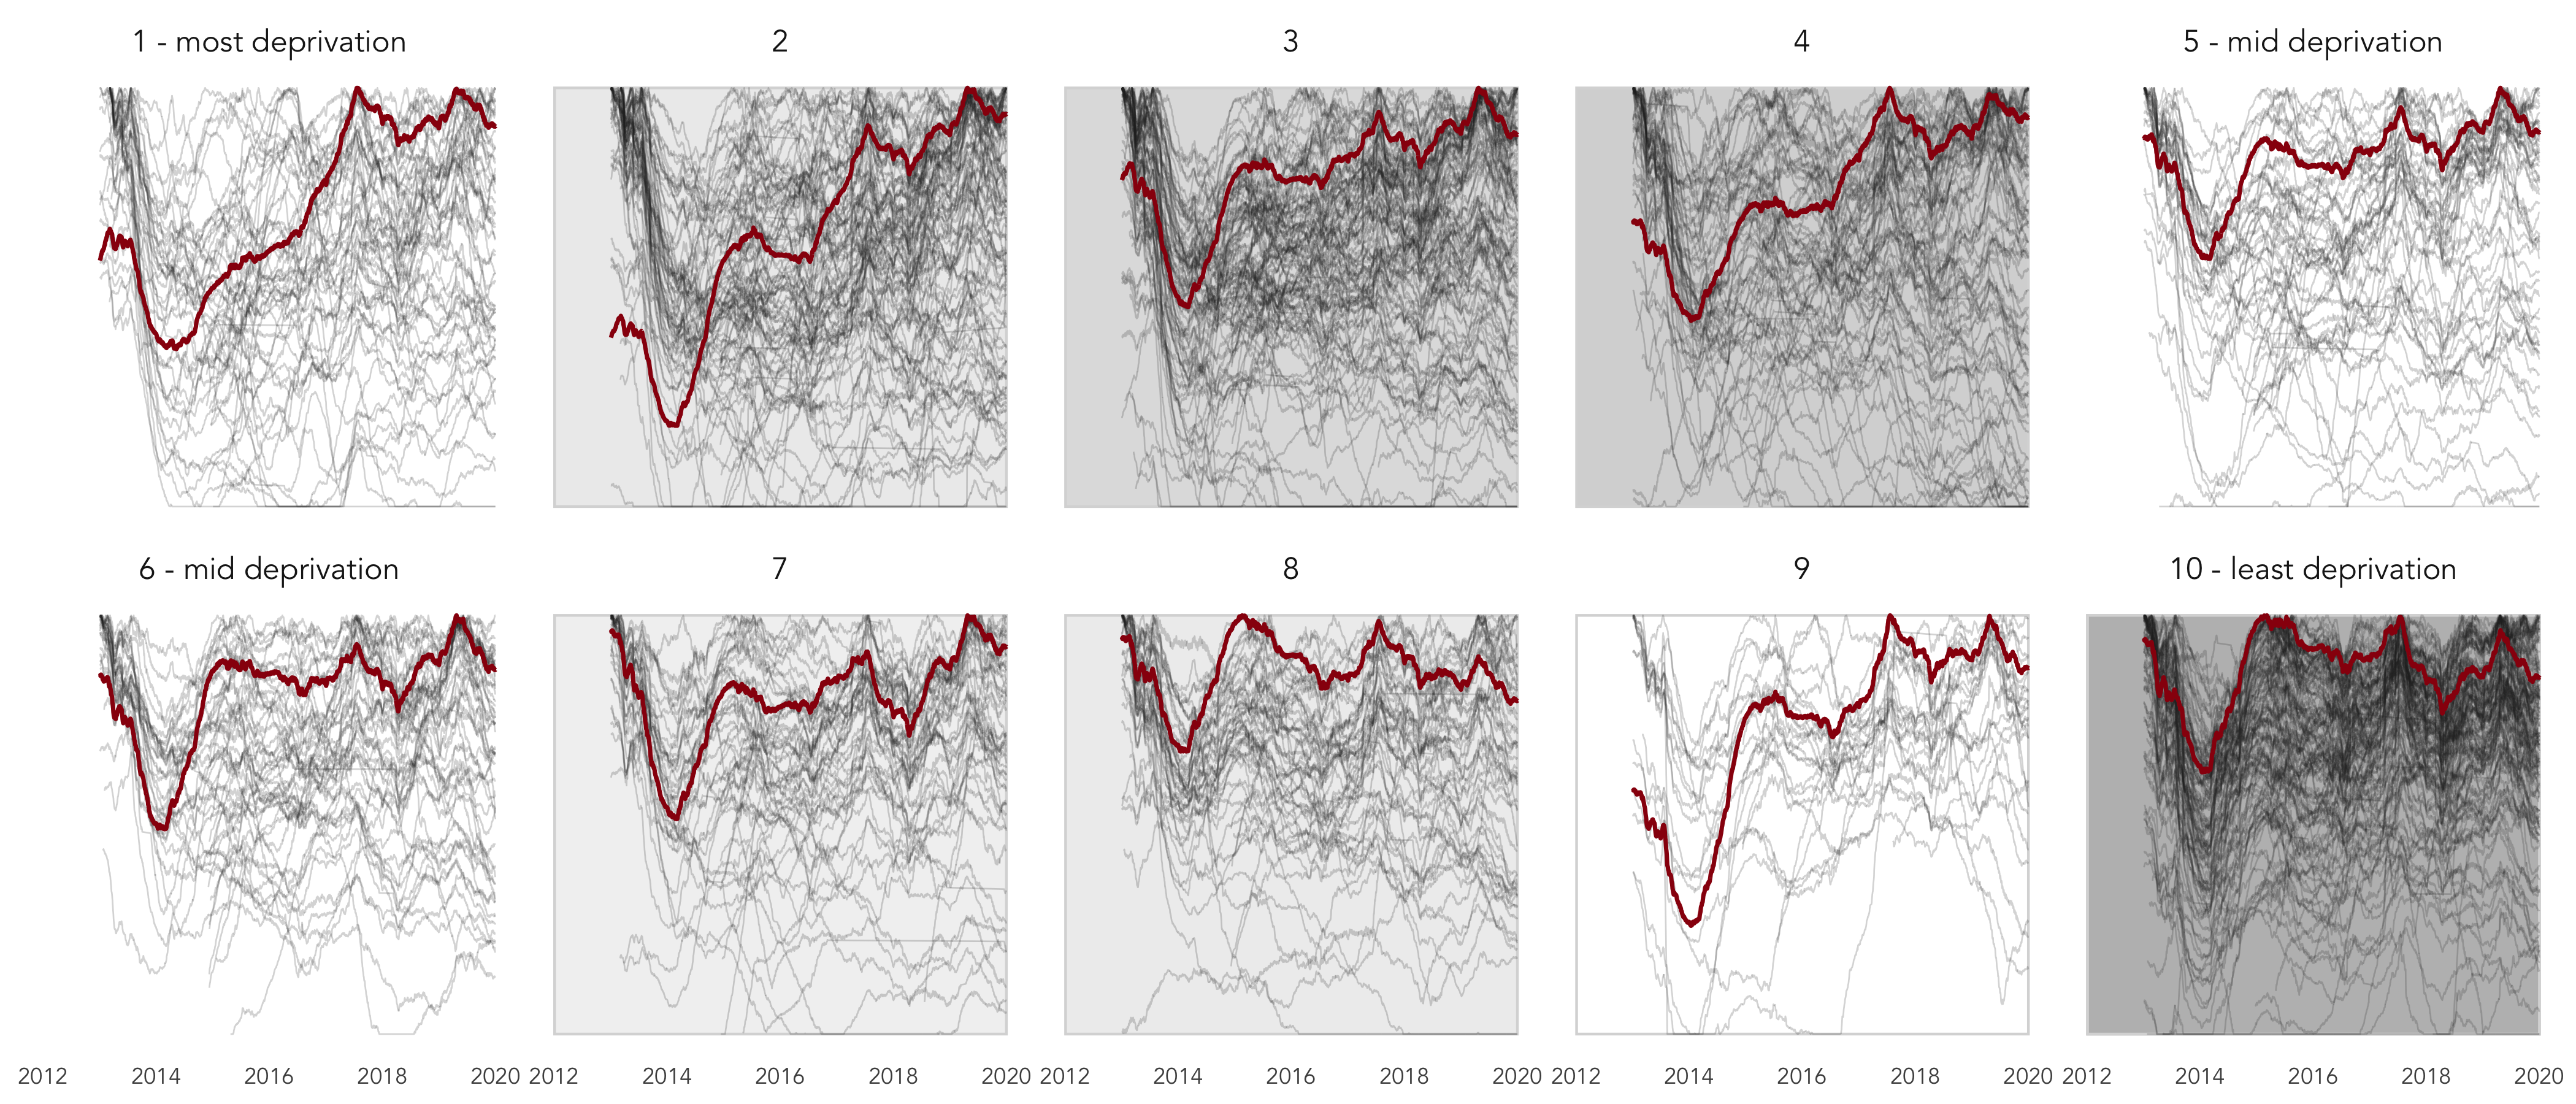
\includegraphics[width=1\linewidth]{figures/daily_hires_station_imd_minor} 

}

\caption{Rolling daily trip counts by income decile (red) and docking stations within income deciles (grey) for 2012-2019. Frequencies are locally scaled by income decile and docking station and with a 365-day smoothing. Docking stations are ordered within small multiples from lowest (1) to highest (10) income deciles. Grey fill within each decile plot varies according to overall trip counts originating from dockin stations in that decile}\label{fig:change-time-income}
\end{figure}

\begin{figure}

{\centering 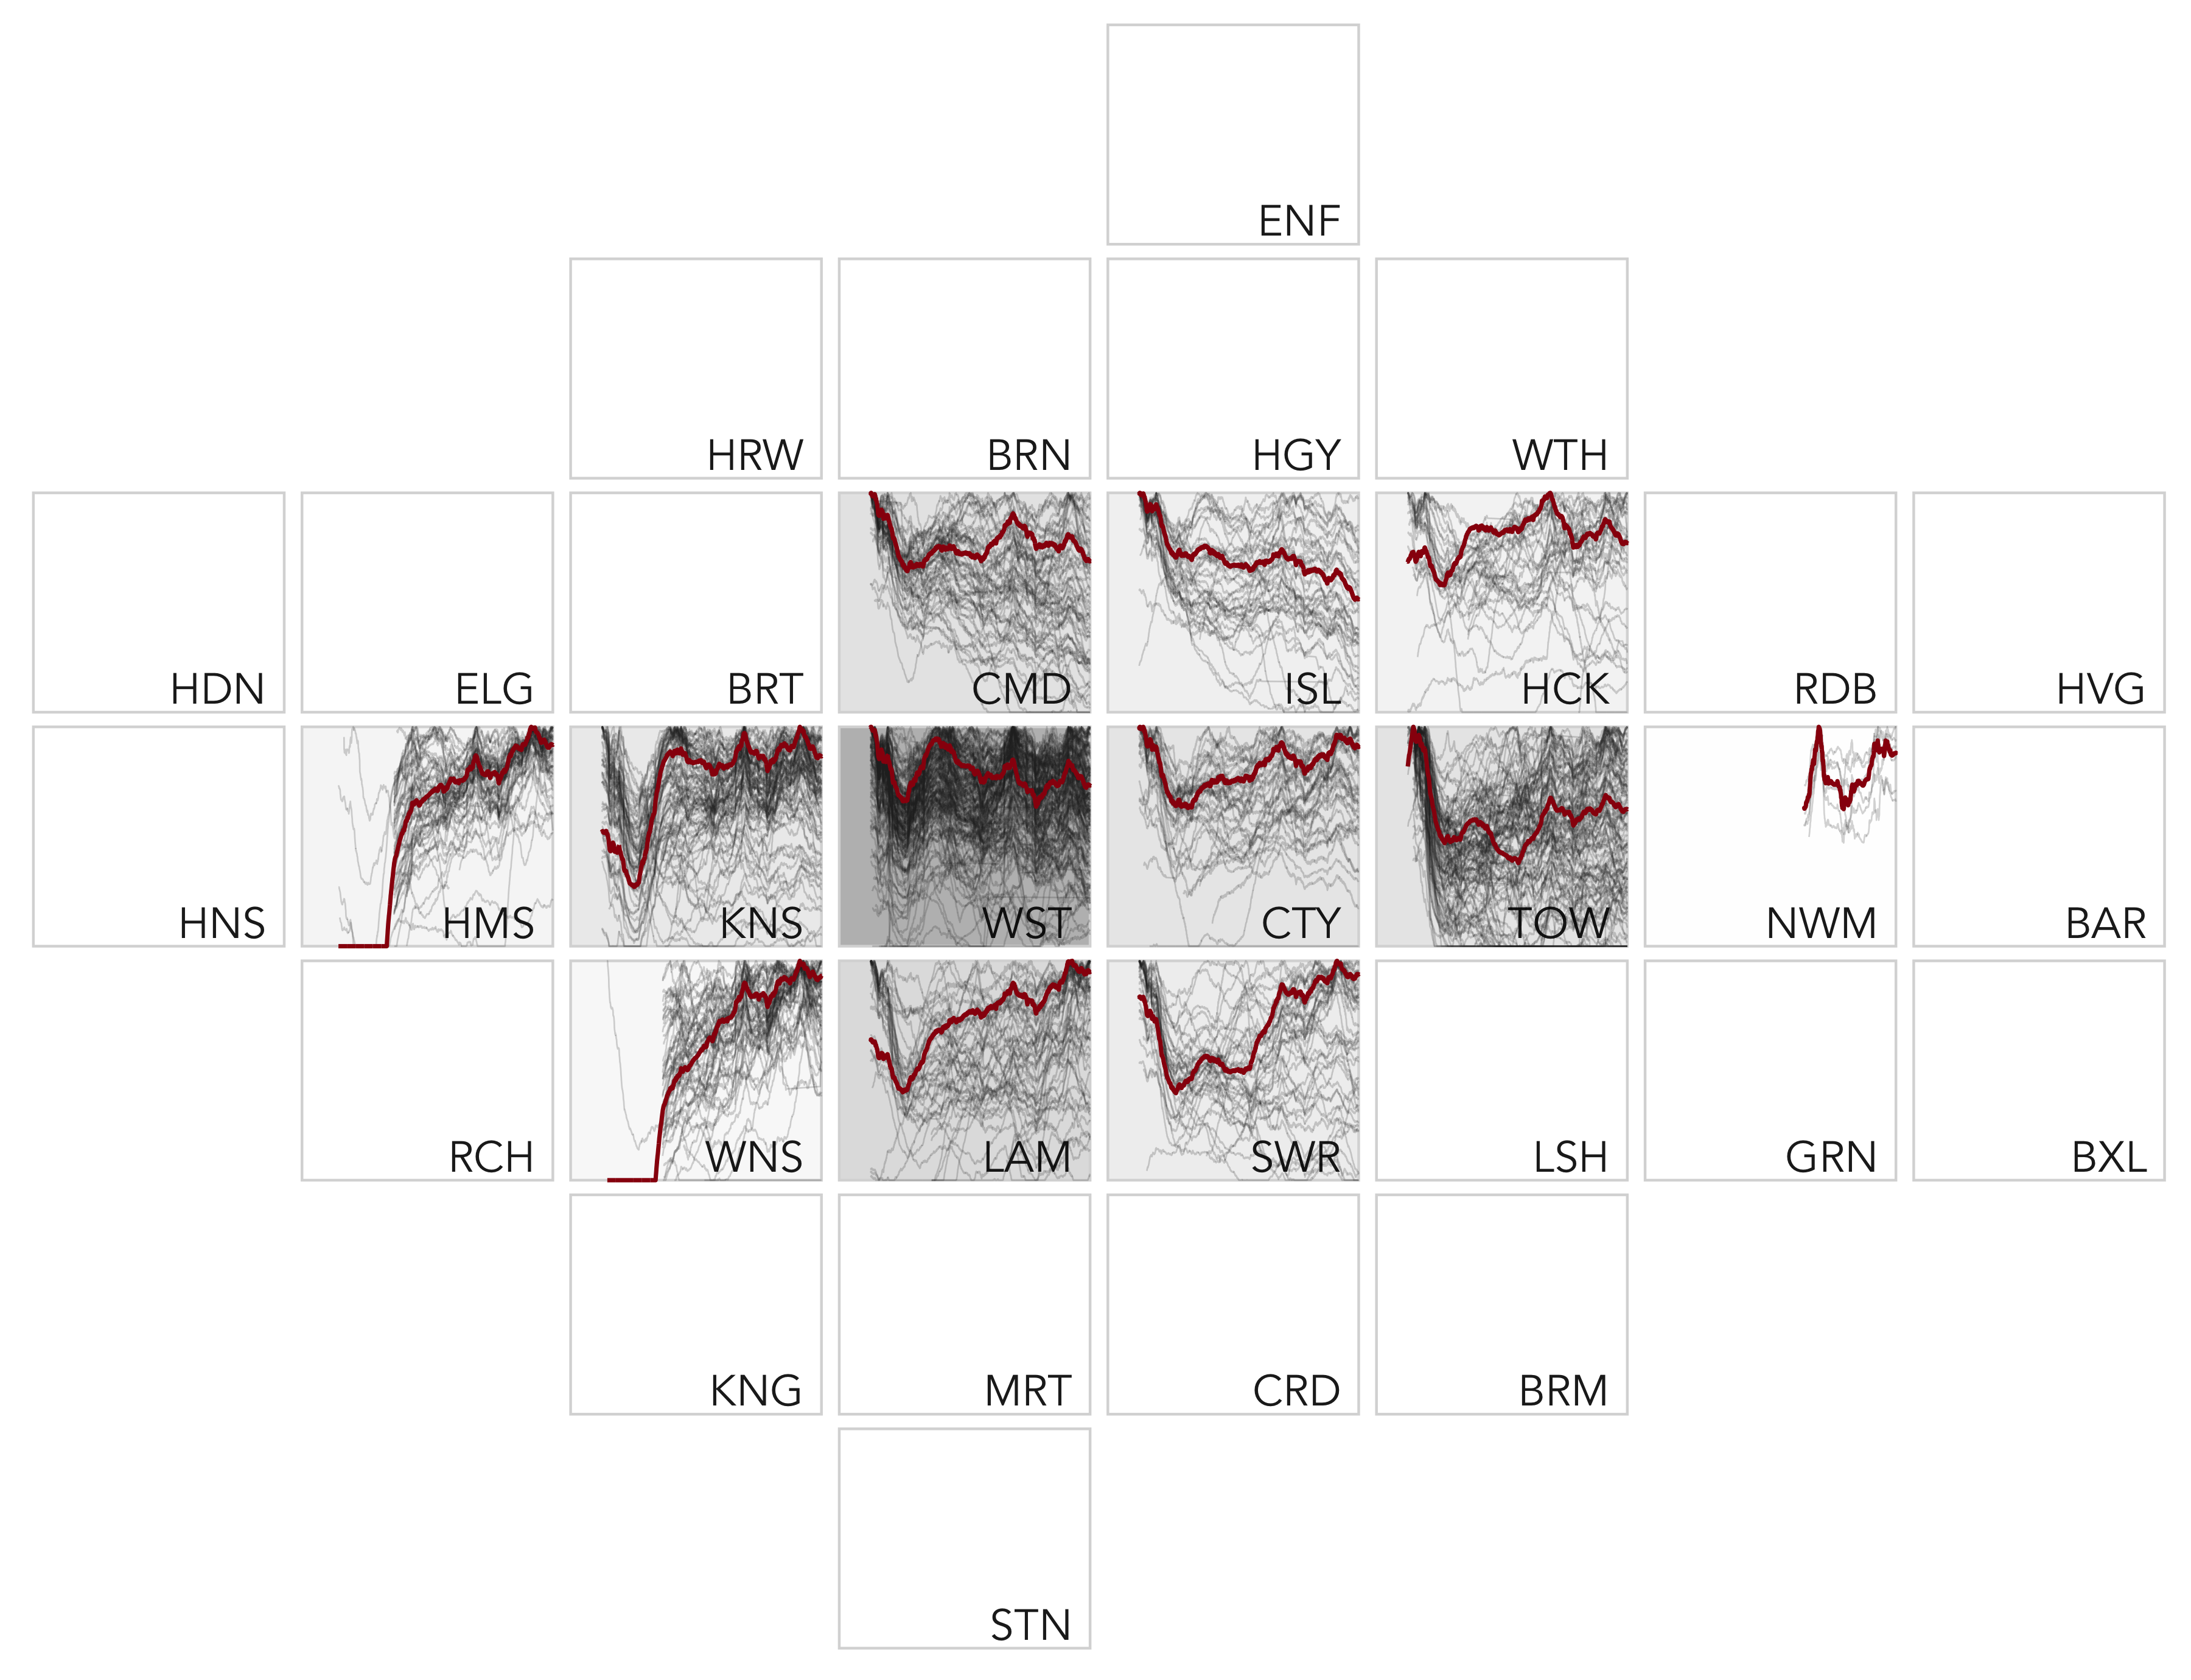
\includegraphics[width=1\linewidth]{figures/daily_hires_station_bor_minor} 

}

\caption{Rolling daily trip counts by London borough (red) and for stations within London boroughs (grey) for 2012-2019. Frequencies are locally scaled by London borough and docking station and with a 365-day smoothing. Docking stations are ordered within small multiples according to the approximate geographic location of London boroughs. Grey fill within each borough varies according to overall trip counts originating from that borough}\label{fig:change-time-boroughs}
\end{figure}

Figure \ref{fig:trip-types-boroughs} shows the temporal trend by time of week: weekday morning (between 0600-1000), weekday evening (between 1600-2100), weekday interpeaks (between 1000-1600), night-time trips (between 2100-0600) and weekend daytime trips (between 0600-2100). Evenings are the dominant trip type for docking stations in job-rich high income boroughs such as City of London and, to a lesser extent, Westminster, Islington, Camden and Southwark.
For docking stations located in boroughs towards the edge of ``prime'' London, morning trips dominate.
This can be largely explained by commuting behaviour.
However, an increasing pattern of morning peak-time journeys is present for boroughs that contain large resident populations and that are not located at a major rail hub (docking stations in Wandsworth and Hackney), suggesting that the use of the LCHS by resident commuters is increasing.
Furthermore, docking stations in these and non-central London boroughs (Kingston, Hammersmith and Tower Hamlets) are associated with large and increasing numbers of weekend trips, suggesting that use of the scheme for \emph{leisure} trips may not merely be the preserve of tourists.

\begin{figure}

{\centering 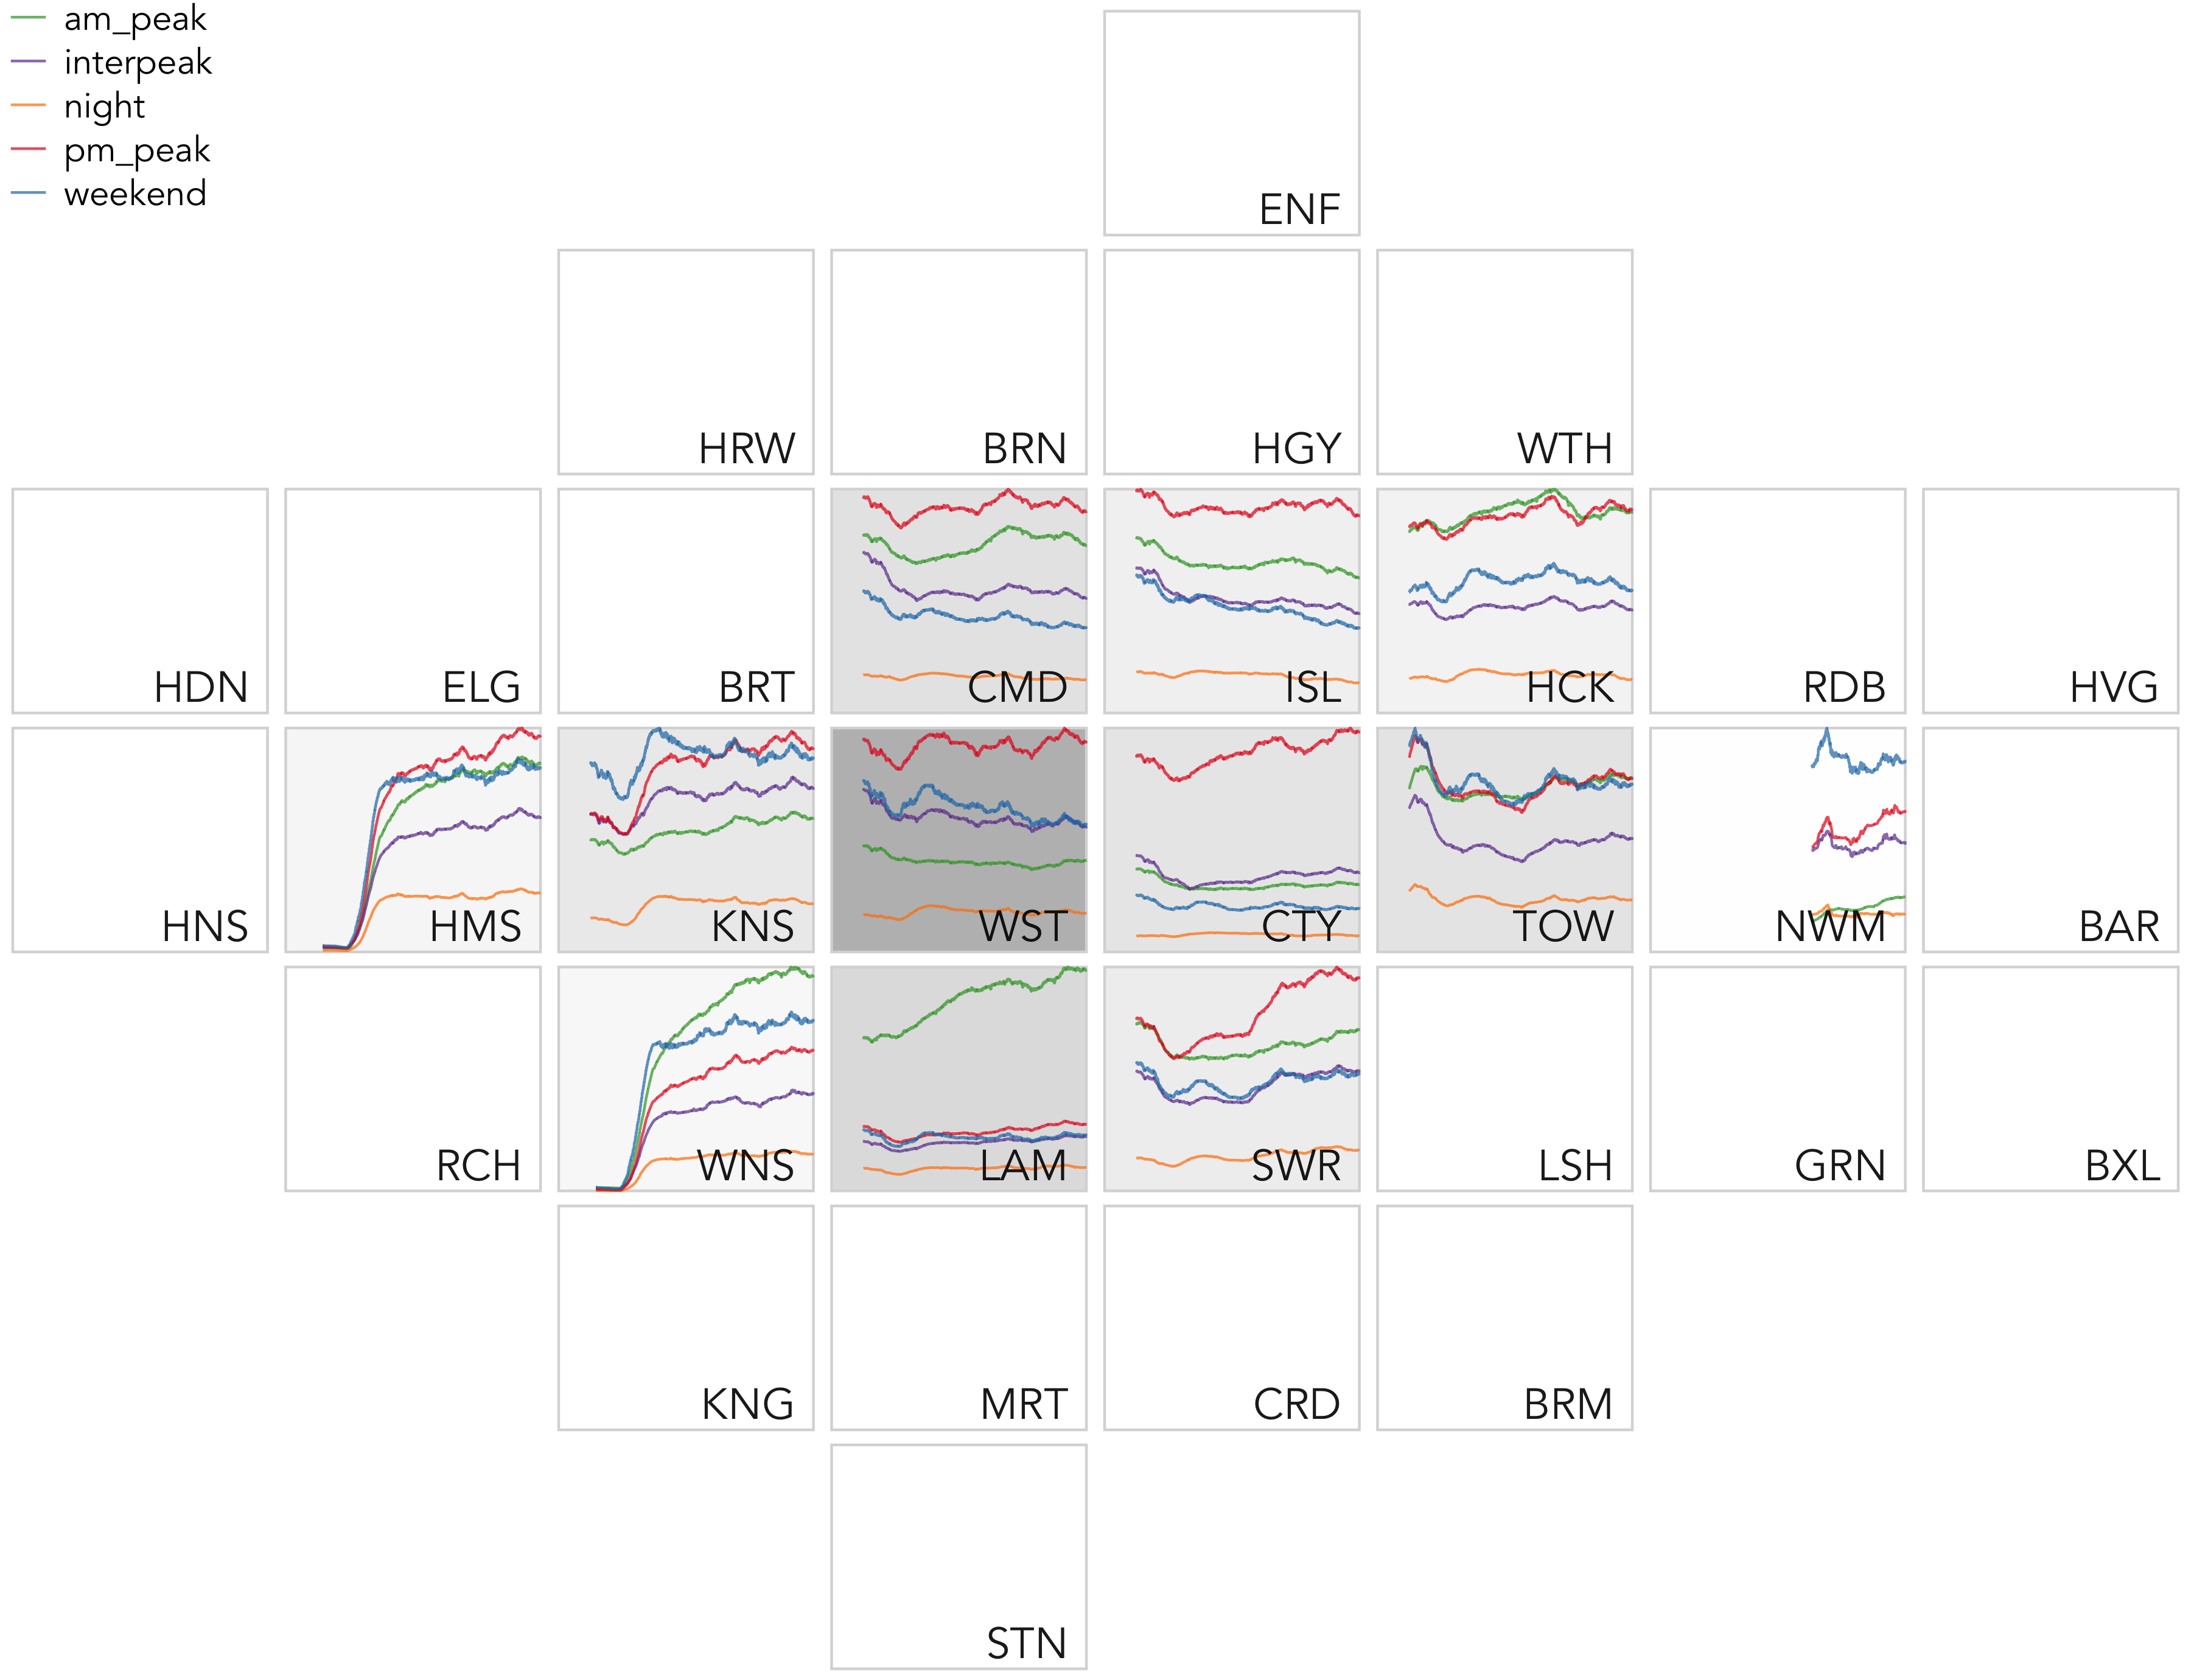
\includegraphics[width=1\linewidth]{figures/trip_types_by_borough_minor} 

}

\caption{Rolling daily trip counts by trip type in London boroughs for 2012-2019. Frequencies are locally scaled by London borough and with a 365-day smoothing. Small multiples are ordered according to the approximate geographic location of London boroughs. Grey fill within each borough varies according to overall trip counts originating from that borough}\label{fig:trip-types-boroughs}
\end{figure}

\hypertarget{discussion}{%
\section{Discussion}\label{discussion}}

We found evidence of growth in bikeshare usage following expansion of the LCHS, including in docking stations located in residential and low income areas.
This suggests that the popularity cycle hire in London is due to its utility:
the `novelty effect' (Mattson and Godavarthy 2017) will have worn off after the first few years (although there could be a residual novelty effect for new docking stations).
The expansion of the LCHS into new areas made the provision of shared mobility more representative of the socio-economic distribution of London as a whole than when the scheme started in wealthier central areas.
Increased availability of cycle hire opportunities to a more diverse range of areas provides an opportunity to test the hypothesis that most cycle hire usage and growth would be in relatively wealthy areas, as reported by Noland (2018), for example.
Contrary to this hypothesis, derived from research in the USA, we found that usage of bikeshare in London was relatively balanced across areas, independent of levels of income deprivation.

Time series plots disaggregated by income decile and geographic location revealed that much of the growth in the usage of the scheme since the expansion into more residential areas has come from relatively low income areas.
The \emph{relatively} higher income deprivation boroughs of Lambeth and Southwark have, for example, experienced high rates of growth compared with areas in Westminster and Kensington, especially during the morning rush hour when users are most likely to be local residents.
The conclusion that we take from the research (expanded on in the next section) is that shared mobility policies, and BSS in particular, can succeed in low income areas.

There are some limitations to the study that should be considered before attempting to generalise the findings, however.
The first limitation relates to the level of analysis: although the geographic resolution of analysis was relatively high (each LSOA zone contains less than 2000 people), the study lacks demographic data at level of individual bikeshare users.
We know very little about the income (and other) characteristics of users \emph{compared with the demographic profile of their local area}, raising the following question:
Could the high rates of growth in low income areas reflect the behaviour of more affluent people (e.g. `hipsters') living in low income areas?
And how does the emergence of dockless schemes (Li et al. 2019) affect inequalities in access to and use of shared mobility services?

Answers to such questions are outside the scope of this paper.
However, given the consistency of growth in a range of low income areas and considering the finances (£2 for 24 hour bikeshare access vs £4.80+ for a single tube ticket), our hypothesis is that future research will find that people on low incomes \emph{are} using the LCHS and other BSS where provision is evenly distributed geographically, and fairly priced.
Figure \ref{fig:profile-users-lchs} shows that although the income profile of casual users is relatively flat, LCHS members tend to be relatively wealthy, with the majority falling into the £75k+ income category.
Follow-on research could explore the extent to which growth in cycle usage in relatively low income areas is driven by wealthy new members or casual users on low incomes.
Second, although the analysis uses small areas as the basis of the analysis, it is possible that `micro-segregation' (Keddie and Tonkiss 2010), where high income and low income households live streets apart, could in part explain the results, further strengthening the need for follow-up studies based on individual-level surveys building on TNS (2017) and Morton (2018).
Third, although our analysis spanned a wider timeframe than other studies, the 8 years of data are insufficient to draw strong conclusions about the long-term direction of travel, especially as many stations in relatively low income areas are comparatively new.
The true levels of inclusiveness of cycling interventions, including bicycle sharing, schemes will take years to become clear.

Methodological advances could help address the limitations outlined above, suggesting further work to support the generalisation of methods to estimate levels of provision and growth in cycle hire in relatively high and low income areas across different cities.
Although income estimates are rarely available for small areas in cities internationally, new methods for estimating wealth and deprivation (Jean et al. 2016) could support further international comparative research into inequalities in cycle hire schemes.

The use of a `hard' cut-off distance between residential building and docking stations (150 m used in the analysis presented) represents a simplification of real world decision-making: in reality, people choose whether or not to use docking stations based on a range of factors.
The probability of making non motorised trips has been found to vary as a non-linear including route distance and perceived levels of danger on the pedestrian network (Iacono, Krizek, and El-Geneidy 2010).
Developing more sophisticated functions linking docking stations to residential areas, weighted by route attributes, is beyond the scope of the present study but represents a potential area for future research: future work could explore the extent to which docking stations located to minimise walking distances and exposure to busy roads succeed, compared with docking stations in less favourable locations on the transport network.

Although such methodological advances should be able to help explain the results of this paper, and the extent to which they can be applied to other cities, it is important to also recognise the limitations of quantitative methods in understanding the reasons why cycling grows in some places and not others.
A clear example of the importance of `wider boundary' factors that are not conducive to quantitative analysis is the observation that cycling levels have increased in recent years in the relatively hilly yet wealthy and cosmopolitan city of Bristol, while falling in the comparatively deprived city of Hull, where `hard' quantitative factors would suggest cycling should grow (Aldred and Jungnickel 2014).
While such cultural factors and social stigma may be harder to measure, they are not impossible to research using methods such as focus groups, participatory research and individual level surveys including appropriate questions revealing attitudes and identities relating to cycling (Bill et al. 2015; Lois, Moriano, and Rondinella 2015), suggesting further lines of enquiry.

Finally, there is great potential for further technical and software development work, to make cycle hire research more accessible and reproducible.
Building on the experiences of packages such as \textbf{bikedata}, which make transport data more accessible for `citizen science' (Padgham and Ellison 2017), future work could develop tools that automate tedious parts of the analysis, allowing future research to focus on the policy issues rather than the time-consuming yet vital data cleaning and analysis stages in cycle hire research.

\hypertarget{conclusion}{%
\section{Conclusion}\label{conclusion}}

Overall, we find little evidence to support the view, articulated by Chardon (2019), that cycle hire schemes are detrimental to transport equity and inclusiveness.
By contrast, in the case of London, the analysis presented in this paper finds that cycle hire \emph{can} enable sustainable transport alternatives to a wide range of people, potentially reducing geographic transport inequalities.
The extent to which these findings will extend to individual-level analysis of bikeshare users, and to other cities, cannot be answered in this paper.
Recent findings suggests that supplementing policies providing access to shared bikes with \emph{additional support measures} such as cycle training and subsidies for certain groups can help ensure that BSS benefits a broader range of people, including disadvantaged groups (Yates and Whyte 2019).
This raises a wider question: can participation policies help address wider vandalism and stigma issues that can plague BSS, by showing that it is not just for ``white, middle-class men''?

To return to the question in the title of the paper: yes, it seems that the London Cycle Hire Scheme is becoming more inclusive over time, at least in terms of the income distribution of provision and usage based on spatial analysis at high spatial and temporal resolution.
Given the stigma around cycling for some low income groups (Portland State University et al. 2017) this should be seen as a major achievement.
The findings support the expansion of bikeshare into more low income and diverse communities.

However, the research presented in this paper also opens up wider questions.
Is usage of cycle hire becoming more equally distributed across other cities, or is London an exception?
How do inequalities of uptake in cycling compare with inequalities of uptake in car use?
And what role can active transport play in creating transport systems that are accessible to everyone?
Regardless of the answers to these emerging questions, the paper provides a counterpoint to the notion that cycle hire schemes only benefit affluent areas and their populations, and suggests that interventions to expand access into poorer areas of major cities can work.

\hypertarget{references}{%
\section*{References}\label{references}}
\addcontentsline{toc}{section}{References}

\hypertarget{refs}{}
\leavevmode\hypertarget{ref-aldred_why_2014}{}%
Aldred, Rachel, and Katrina Jungnickel. 2014. ``Why Culture Matters for Transport Policy: The Case of Cycling in the UK.'' \emph{Journal of Transport Geography}, no. early: 1--22. \url{http://www.sciencedirect.com/science/article/pii/S0966692313002202}.

\leavevmode\hypertarget{ref-bachand-marleau_better_2012}{}%
Bachand-Marleau, Julie, Brian Lee, and Ahmed El-Geneidy. 2012. ``Better Understanding of Factors Influencing Likelihood of Using Shared Bicycle Systems and Frequency of Use.'' \emph{Transportation Research Record: Journal of the Transportation Research Board} 2314 (December): 66--71. \url{https://doi.org/10.3141/2314-09}.

\leavevmode\hypertarget{ref-bell_soft_2016}{}%
Bell, Emma. 2016. ``Soft Power and Corporate Imperialism: Maintaining British Influence.'' \emph{Race \& Class} 57 (4): 75--86. \url{https://doi.org/10.1177/0306396815624865}.

\leavevmode\hypertarget{ref-bernatchez_knowing_2015}{}%
Bernatchez, Annie C., Lise Gauvin, Daniel Fuller, Anne Sophie Dubé, and Louis Drouin. 2015. ``Knowing About a Public Bicycle Share Program in Montreal, Canada: Are Diffusion of Innovation and Proximity Enough for Equitable Awareness?'' \emph{Journal of Transport \& Health} 2 (3): 360--68. \url{https://doi.org/10.1016/j.jth.2015.04.005}.

\leavevmode\hypertarget{ref-bill_representing_2015}{}%
Bill, E.M., G. Baker, N.S. Ferguson, D. Drinkwater, and N. Mutrie. 2015. ``Representing Active Travel: A Formative Evaluation of a Computer Visualisation Tool Demonstrating a New Walking and Cycling Route.'' \emph{Environment and Planning B: Planning and Design} 42 (3): 450--67. \url{https://doi.org/10.1068/b130155p}.

\leavevmode\hypertarget{ref-buck_are_2013}{}%
Buck, Darren, Ralph Buehler, Patricia Happ, Bradley Rawls, Payton Chung, and Natalie Borecki. 2013. ``Are Bikeshare Users Different from Regular Cyclists?: A First Look at Short-Term Users, Annual Members, and Area Cyclists in the Washington, D.c., Region.'' \emph{Transportation Research Record: Journal of the Transportation Research Board} 2387 (December): 112--19. \url{https://doi.org/10.3141/2387-13}.

\leavevmode\hypertarget{ref-de_chardon_contradictions_2019}{}%
Chardon, Cyrille Medard de. 2019. ``The Contradictions of Bike-Share Benefits, Purposes and Outcomes.'' \emph{Transportation Research Part A: Policy and Practice} 121: 401--19.

\leavevmode\hypertarget{ref-clark_bicycle_2016}{}%
Clark, Julie, and Angela Curl. 2016. ``Bicycle and Car Share Schemes as Inclusive Modes of Travel? A Socio-Spatial Analysis in Glasgow, UK.'' \emph{Social Inclusion} 4 (3): 83. \url{https://doi.org/10.17645/si.v4i3.510}.

\leavevmode\hypertarget{ref-daddio_maximizing_2012}{}%
Daddio, David William, and N. Mcdonald. 2012. ``Maximizing Bicycle Sharing: An Empirical Analysis of Capital Bikeshare Usage.'' \emph{University of North Carolina at Chapel Hill} 8.

\leavevmode\hypertarget{ref-didonato_city-bike_2002}{}%
DiDonato, Michael, Stephen Herbert, and D. Vachhani. 2002. ``City-Bike Maintenance and Availability.'' \emph{Project Report (Project No. 44-JSD-DPC3). Worcester Polytechnic Institute. Neuvedeno}.

\leavevmode\hypertarget{ref-duran_bicycle-sharing_2018}{}%
Duran, Ana Clara, Esther Anaya-Boig, Joshua Daniel Shake, Leandro Martin Totaro Garcia, Leandro Fórnias Machado de Rezende, and Thiago Hérick de Sá. 2018. ``Bicycle-Sharing System Socio-Spatial Inequalities in Brazil.'' \emph{Journal of Transport \& Health} 8 (March): 262--70. \url{https://doi.org/10.1016/j.jth.2017.12.011}.

\leavevmode\hypertarget{ref-fishman_bikeshare:_2016}{}%
Fishman, Elliot. 2016. ``Bikeshare: A Review of Recent Literature.'' \emph{Transport Reviews} 36 (1): 92--113. \url{https://doi.org/10.1080/01441647.2015.1033036}.

\leavevmode\hypertarget{ref-fishman_safety_2018}{}%
Fishman, Elliot, and Paul Schepers. 2018. ``The Safety of Bike Share Systems.'' OECD. \url{https://www.oecd-ilibrary.org/transport/the-safety-of-bike-share-systems_acf28971-en}.

\leavevmode\hypertarget{ref-fishman_bike_2013}{}%
Fishman, Elliot, Simon Washington, and Narelle Haworth. 2013. ``Bike Share: A Synthesis of the Literature.'' \emph{Transport Reviews} 33 (2): 148--65. \url{https://doi.org/10.1080/01441647.2013.775612}.

\leavevmode\hypertarget{ref-fishman_bike_2014}{}%
---------. 2014. ``Bike Share's Impact on Car Use: Evidence from the United States, Great Britain, and Australia.'' \emph{Transportation Research Part D: Transport and Environment} 31 (August): 13--20. \url{https://doi.org/10.1016/j.trd.2014.05.013}.

\leavevmode\hypertarget{ref-fuller_use_2011}{}%
Fuller, Daniel, Lise Gauvin, Yan Kestens, Mark Daniel, Michel Fournier, Patrick Morency, and Louis Drouin. 2011. ``Use of a New Public Bicycle Share Program in Montreal, Canada.'' \emph{American Journal of Preventive Medicine} 41 (1): 80--83. \url{https://doi.org/10.1016/j.amepre.2011.03.002}.

\leavevmode\hypertarget{ref-goodman_role_2014}{}%
Goodman, Anna, Judith Green, and James Woodcock. 2014. ``The Role of Bicycle Sharing Systems in Normalising the Image of Cycling: An Observational Study of London Cyclists.'' \emph{Journal of Transport \& Health} 1 (1): 5--8. \url{https://doi.org/10.1016/j.jth.2013.07.001}.

\leavevmode\hypertarget{ref-greater_london_authority_mayors_2010}{}%
Greater London Authority. 2010. ``The Mayor's Transport Strategy.'' GLA London. \url{https://infrastructure.planninginspectorate.gov.uk/wp-content/ipc/uploads/projects/TR010021/TR010021-000409-Mayor\%27s\%20Transport\%20Strategy.pdf}.

\leavevmode\hypertarget{ref-hampshire_analysis_2012}{}%
Hampshire, Robert C., and Lavanya Marla. 2012. ``An Analysis of Bike Sharing Usage: Explaining Trip Generation and Attraction from Observed Demand.'' In \emph{91st Annual Meeting of the Transportation Research Board, Washington, DC}, 12--2099.

\leavevmode\hypertarget{ref-heinen_public_2018}{}%
Heinen, Eva, Md. Kamruzzaman, and Gavin Turrell. 2018. ``The Public Bicycle-Sharing Scheme in Brisbane, Australia: Evaluating the Influence of Its Introduction on Changes in Time Spent Cycling Amongst a Middle- and Older-Age Population.'' \emph{Journal of Transport \& Health} 10 (September): 56--73. \url{https://doi.org/10.1016/j.jth.2018.07.003}.

\leavevmode\hypertarget{ref-heinen_commuting_2010}{}%
Heinen, Eva, Bert van Wee, and Kees Maat. 2010. ``Commuting by Bicycle: An Overview of the Literature.'' \emph{Transport Reviews} 30 (1): 59--96. \url{https://doi.org/10.1080/01441640903187001}.

\leavevmode\hypertarget{ref-hosford_who_2018}{}%
Hosford, Kate, and Meghan Winters. 2018. ``Who Are Public Bicycle Share Programs Serving? An Evaluation of the Equity of Spatial Access to Bicycle Share Service Areas in Canadian Cities.'' \emph{Transportation Research Record} 2672 (36): 42--50. \url{https://doi.org/10.1177/0361198118783107}.

\leavevmode\hypertarget{ref-iacono_measuring_2010}{}%
Iacono, Michael, Kevin J. Krizek, and Ahmed El-Geneidy. 2010. ``Measuring Non-Motorized Accessibility: Issues, Alternatives, and Execution.'' \emph{Journal of Transport Geography} 18 (1): 133--40. \url{https://doi.org/10.1016/j.jtrangeo.2009.02.002}.

\leavevmode\hypertarget{ref-jean_combining_2016}{}%
Jean, Neal, Marshall Burke, Michael Xie, W. Matthew Davis, David B. Lobell, and Stefano Ermon. 2016. ``Combining Satellite Imagery and Machine Learning to Predict Poverty.'' \emph{Science} 353 (6301). American Association for the Advancement of Science: 790--94.

\leavevmode\hypertarget{ref-keddie_market_2010}{}%
Keddie, Jamie, and Fran Tonkiss. 2010. ``The Market and the Plan: Housing, Urban Renewal and Socio-Economic Change in London.'' \emph{City, Culture and Society} 1 (2): 57--67.

\leavevmode\hypertarget{ref-league_of_american_bicyclists_new_2015}{}%
League of American Bicyclists, and Sierra Club. 2015. ``The New Majority - Pedalling Towards Equity.'' Sierra Club. \url{https://www.bikeleague.org/sites/default/files/equity_report.pdf}.

\leavevmode\hypertarget{ref-li_effects_2019}{}%
Li, Haojie, Yingheng Zhang, Hongliang Ding, and Gang Ren. 2019. ``Effects of Dockless Bike-Sharing Systems on the Usage of the London Cycle Hire.'' \emph{Transportation Research Part A: Policy and Practice} 130 (December): 398--411. \url{https://doi.org/10.1016/j.tra.2019.09.050}.

\leavevmode\hypertarget{ref-lois_cycle_2015}{}%
Lois, David, Juan Antonio Moriano, and Gianni Rondinella. 2015. ``Cycle Commuting Intention: A Model Based on Theory of Planned Behaviour and Social Identity.'' \emph{Transportation Research Part F: Traffic Psychology and Behaviour} 32: 101--13.

\leavevmode\hypertarget{ref-mattson_bike_2017}{}%
Mattson, Jeremy, and Ranjit Godavarthy. 2017. ``Bike Share in Fargo, North Dakota: Keys to Success and Factors Affecting Ridership.'' \emph{Sustainable Cities and Society} 34 (October): 174--82. \url{https://doi.org/10.1016/j.scs.2017.07.001}.

\leavevmode\hypertarget{ref-mooney_freedom_2019}{}%
Mooney, Stephen J., Kate Hosford, Bill Howe, An Yan, Meghan Winters, Alon Bassok, and Jana A. Hirsch. 2019. ``Freedom from the Station: Spatial Equity in Access to Dockless Bike Share.'' \emph{Journal of Transport Geography} 74 (January): 91--96. \url{https://doi.org/10.1016/j.jtrangeo.2018.11.009}.

\leavevmode\hypertarget{ref-morton_appraising_2018}{}%
Morton, Craig. 2018. ``Appraising the Market for Bicycle Sharing Schemes: Perceived Service Quality, Satisfaction, and Behavioural Intention in London.'' \emph{Case Studies on Transport Policy} 6 (1): 102--11. \url{https://doi.org/10.1016/j.cstp.2017.11.003}.

\leavevmode\hypertarget{ref-nair_large-scale_2013}{}%
Nair, Rahul, Elise Miller-Hooks, Robert C. Hampshire, and Ana Bušić. 2013. ``Large-Scale Vehicle Sharing Systems: Analysis of Vélib'.'' \emph{International Journal of Sustainable Transportation} 7 (1): 85--106.

\leavevmode\hypertarget{ref-nikitas_how_2019}{}%
Nikitas, Alexandros. 2019. ``How to Save Bike-Sharing: An Evidence-Based Survival Toolkit for Policy-Makers and Mobility Providers.'' \emph{Sustainability} 11 (11): 3206.

\leavevmode\hypertarget{ref-noland_bikesharing_2018}{}%
Noland, Robert B. 2018. ``Bikesharing in Philadelphia - Do Lower-Income Areas Generate Trips.''

\leavevmode\hypertarget{ref-obrien_mining_2014}{}%
O'Brien, Oliver, James Cheshire, Michael Batty, and Oliver O'Brien. 2014. ``Mining Bicycle Sharing Data for Generating Insights into Sustainable Transport Systems.'' \emph{Journal of Transport Geography} 34 (July): 262--73. \url{https://doi.org/10.1016/j.jtrangeo.2013.06.007}.

\leavevmode\hypertarget{ref-ogilvie_inequalities_2012}{}%
Ogilvie, F., and A. Goodman. 2012. ``Inequalities in Usage of a Public Bicycle Sharing Scheme: Socio-Demographic Predictors of Uptake and Usage of the London (UK) Cycle Hire Scheme.'' \emph{Preventive Medicine} 55 (1): 40--45. \url{https://doi.org/10.1016/j.ypmed.2012.05.002}.

\leavevmode\hypertarget{ref-padgham_bikedata:_2017}{}%
Padgham, Mark, and Richard Ellison. 2017. \emph{Bikedata: Download and Aggregate Data from Public Hire Bicycle Systems}. \url{https://CRAN.R-project.org/package=bikedata}.

\leavevmode\hypertarget{ref-pebesma_simple_2018}{}%
Pebesma, Edzer. 2018. ``Simple Features for R: Standardized Support for Spatial Vector Data.'' \emph{The R Journal}.

\leavevmode\hypertarget{ref-portland_state_university_breaking_2017}{}%
Portland State University, Nathan McNeil, Jennifer Dill, John MacArthur, Joseph Broach, and Steven Howland. 2017. ``Breaking Barriers to Bike Share: Insights from Residents of Traditionally Underserved Neighborhoods.'' Portland State University. \url{https://doi.org/10.15760/trec.176}.

\leavevmode\hypertarget{ref-R-base}{}%
R Core Team. 2020. \emph{R: A Language and Environment for Statistical Computing}. Vienna, Austria: R Foundation for Statistical Computing.

\leavevmode\hypertarget{ref-ricci_bike_2015}{}%
Ricci, Miriam. 2015. ``Bike Sharing: A Review of Evidence on Impacts and Processes of Implementation and Operation.'' \emph{Research in Transportation Business \& Management} 15 (June): 28--38. \url{https://doi.org/10.1016/j.rtbm.2015.03.003}.

\leavevmode\hypertarget{ref-rixey_station-level_2013}{}%
Rixey, R. Alexander. 2013. ``Station-Level Forecasting of Bikesharing Ridership: Station Network Effects in Three US Systems.'' \emph{Transportation Research Record} 2387 (1): 46--55.

\leavevmode\hypertarget{ref-shaheen_bikesharing_2012}{}%
Shaheen, Susan, Stacey Guzman, and Hua Zhang. 2012. ``Bikesharing Across the Globe.'' \emph{Pucher J, Buehler R. Eds}, 183--209.

\leavevmode\hypertarget{ref-shrubsole_who_2019}{}%
Shrubsole, Guy. 2019. \emph{Who Owns England?: How We Lost Our Green and Pleasant Land, and How to Take It Back}. London: William Collins.

\leavevmode\hypertarget{ref-soltani_exploring_2019}{}%
Soltani, Ali, Tamás Mátrai, Rosalia Camporeale, and Andrew Allan. 2019. ``Exploring Shared-Bike Travel Patterns Using Big Data: Evidence in Chicago and Budapest.'' In \emph{International Conference on Computers in Urban Planning and Urban Management}, 53--68. Springer.

\leavevmode\hypertarget{ref-sustrans_our_2019}{}%
Sustrans. 2019. ``Our Position on Public Cycle Share Schemes. Sustrans.'' 2019. \url{https://www.sustrans.org.uk/our-blog/policy-positions/all/all/our-position-on-public-cycle-share-schemes/}.

\leavevmode\hypertarget{ref-tfl_santander_2016}{}%
TfL. 2016. ``Santander Cycles Casual Users Profile - Q2 2015/16.'' Transport for London. \url{http://content.tfl.gov.uk/santander-cycles-casuals.pdf}.

\leavevmode\hypertarget{ref-tns_santander_2017}{}%
TNS. 2017. ``Santander Cycles Customer Satisfaction and Usage Survey Casual Users Only: Quarter 2 2017/18.'' \url{http://content.tfl.gov.uk/santander-cycles-casuals-css-q2-2017-18.pdf}.

\leavevmode\hypertarget{ref-transport_for_london_cycling_2010}{}%
Transport for London. 2010. ``Cycling Revolution London.'' Transport for London. \url{https://www.london.gov.uk/sites/default/files/cycling-revolution-london.pdf}.

\leavevmode\hypertarget{ref-ursaki_quantifying_2015}{}%
Ursaki, Julia, and Lisa Aultman-Hall. 2015. ``Quantifying the Equity of Bikeshare Access in US Cities.'' University of Vermont Transportation Research Center.

\leavevmode\hypertarget{ref-wang_new_2019}{}%
Wang, Jueyu, and Greg Lindsey. 2019. ``Do New Bike Share Stations Increase Member Use: A Quasi-Experimental Study.'' \emph{Transportation Research Part A: Policy and Practice} 121 (March): 1--11. \url{https://doi.org/10.1016/j.tra.2019.01.004}.

\leavevmode\hypertarget{ref-ggplot2}{}%
Wickham, Hadley. 2016. \emph{Ggplot2: Elegant Graphics for Data Analysis}. Springer-Verlag New York. \url{https://ggplot2.tidyverse.org}.

\leavevmode\hypertarget{ref-yates_bikes_2019}{}%
Yates, Gregor, and Bruce Whyte. 2019. ``Bikes for All: Widening Access to Cycling Through Social Inclusion.'' Glasgow Centre for Population Health. \url{https://como.org.uk/wp-content/uploads/2019/11/Bike-for-All-Summary-Report-A4-Final-Draft.pdf}.

\leavevmode\hypertarget{ref-zhang_expanding_2016}{}%
Zhang, Ying, Tom Thomas, M. J. G. Brussel, and MFAM Van Maarseveen. 2016. ``Expanding Bicycle-Sharing Systems: Lessons Learnt from an Analysis of Usage.'' \emph{PLoS One} 11 (12): e0168604.

\leavevmode\hypertarget{ref-zhao_effect_2019}{}%
Zhao, De, Ghim Ping Ong, Wei Wang, and Xiao Jian Hu. 2019. ``Effect of Built Environment on Shared Bicycle Reallocation: A Case Study on Nanjing, China.'' \emph{Transportation Research Part A: Policy and Practice} 128 (October): 73--88. \url{https://doi.org/10.1016/j.tra.2019.07.018}.

\end{document}
